\documentclass{article}
\usepackage{jheppub}
\usepackage{amsmath}
\usepackage{graphicx}
\usepackage{amssymb}
\usepackage{subfig}
\usepackage{natbib}
\bibliographystyle{JHEP-2}
\usepackage[utf8]{inputenc}

\title{Jet-Images -- Deep Learning Edition}
\author{Luke de Oliveira,${}^a$}
\author{Michael Kagan,${}^{b}$}
\author{Lester Mackey,${}^c$}
\author{Benjamin Nachman,${}^{b}$ and}
\author{Ariel Schwartzman${}^b$}

\affiliation{$^{a}$ Institute for Computational and Mathematical Engineering, Stanford University, Stanford, CA 94305, USA}

\affiliation{$^{b}$SLAC National Accelerator Laboratory, Stanford University, 2575 Sand Hill Rd, Menlo Park,
  CA 94025, U.S.A.}

\affiliation{$^{a}$Department of Statistics, Stanford University, Stanford, CA 94305, USA}

\emailAdd{lukedeo@stanford.edu, mkatan@cern.ch, lmackey@stanford.edu, bnachman@cern.ch, sch@slac.stanford.edu}

\abstract{Building on the notion of a particle physics detector as a camera and the collimated streams of high energy particles it measures as an image, we investigate the potential of machine learning techniques based on deep learning architectures.  Modern deep learning algorithms trained on {\it jet images} can out-perform standard physically-motivated feature driven approaches to jet tagging.  We develop techniques for visualizing where these features are learned by the network and what additional information is used to improve performance. This feedback loop between physically-motivated feature driven tools and unsupervised learning algorithms is general and can be used to significantly increase the sensitivity to discover new particles and new forces.}

\begin{document}

\maketitle

\section{Introduction}

The fundamental challenge at the energy frontier of particle physics is identifying subtle signals beneath enormous backgrounds. A monumental triumph was the recent discovery of the Higgs boson - a particle that is produced one in every $10^{10}$ collisions at the Large Hadron Collider (LHC). Machine learning techniques have played a key role in all aspects of this search.  At the most basic level, charged particle tracks are reconstructed using pattern recognition techniques, higher level objects, blah blah. 

Techniques built on physically motivated features have succesfully probed the highest energies and smallest scales ever achieved in terestrial experiments.  At the same time, there have been significant gains 

The high particle multiplicity final states of hadron collider events 
Something like "we have figured out many cool variables" "machine learning can find variables"  "lets use one to inform/improve the other!"

Places where ML is used in HEP: TMVA~\cite{Hocker:2007ht}

b-tagging: MV1 (ATLAS) and CSV (CMS)
tau-tagging
NP searches
rare SM measurements (e.g. single top)
Higgs

Jet Images paper: http://arxiv.org/abs/1407.5675


Let's keep a running document with all pub-ready plots in here.


\section{Simulation Details}
\label{sec:simulation}

In order to study jet images in a realistic scenario, we use Monte Carlo (MC) simulations of high energy particle collisions. One important jet tagging task is to distinguish the hadronic decays of high $p_T$ $W$ bosons from generic SM background processes computes of quarks and gluons.  To simulate high $p_T$ $W$ bosons, a hypothetical $W'$ boson is generated and forced to decay to a hadronically decaying $W$ boson and a $Z$ boson which decays invisibly.


Two physics processes are generated using \textsc{Pythia} 8.170~\cite{Pythia8,Pythia} at $\sqrt{s}=14$ TeV.   To simulate high $p_T$ hadronic $W$ decays, $W'$ bosons are generated to decay exclusively into a $W(\rightarrow qq')$ and $Z(\rightarrow\nu\nu)$.  The $p_T$ scale of the hadronically decaying $W$ is set by the mass of the $W'$ which is tuned to 600 and 800~GeV for this study so that the $200$ GeV $\lesssim p_T^W \lesssim 400$ GeV. In this $p_T^W$ range, the $W$ decay products are expected to merge within a cone of $R~1.0$ where $\Delta R^2=\Delta\phi^2+\Delta\eta^2\sim 4m_W^2/p_{T,W}^2$.  To study the impact on signal versus background, QCD dijets are generated with a range of $\hat{p}_T$ that is approximately in the same range as the relevant signal process.  Anti-$k_t$ jets are clustered using \textsc{FastJet}~\cite{fastjet} 3.0.3.  The signal processes are chosen such that jets with radius parameter $R = 1$ are most appropriate in capturing the decay products of the heavy particles.  The anti-$k_t$ jets are trimmed~\cite{trimming} by re-clustering the constituents into $R=0.3$ $k_t$ subjets and dropping those which have $p_T^\text{subjet}<0.05\times p_T^\text{jet}$. 

To model the discretization and finite acceptance of a real detector, a calorimeter of towers with size $0.1\times 0.1$ in $(y,\phi)$ extends out to $y=5.0$.  The total energy of the simulated particles incident upon a particular cell are added as scalars and the four-vector $p_j$ of any particular tower $j$ is given by

\begin{align}
\label{eq:calo}
p_j = \sum_{i\text{ incident on $j$}}E_i(\cos\phi_j/\cosh y_j,\sin\phi_j/\cosh y_j,\sinh y_j/\cosh y_j,1).
\end{align}


\begin{figure}[bt]
  \begin{center}
      \subfloat[Unweighted $p_T$ distribution \label{subfig:unweighted_pt}]{
        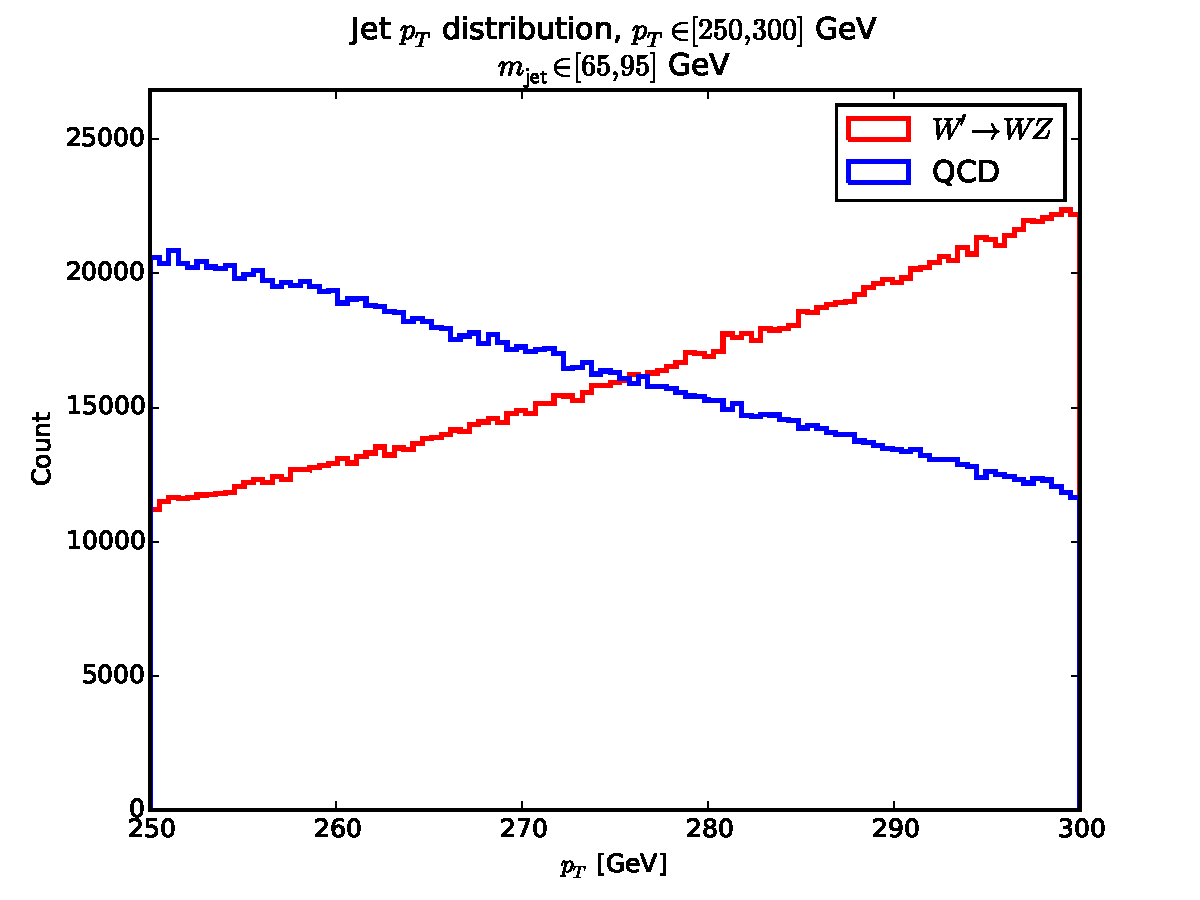
\includegraphics[width=0.5\textwidth]{figures/unweighted-pt-distribution-[250-300].pdf}
      }
      \subfloat[Weighted $p_T$ distribution \label{subfig:weighted_pt}]{
        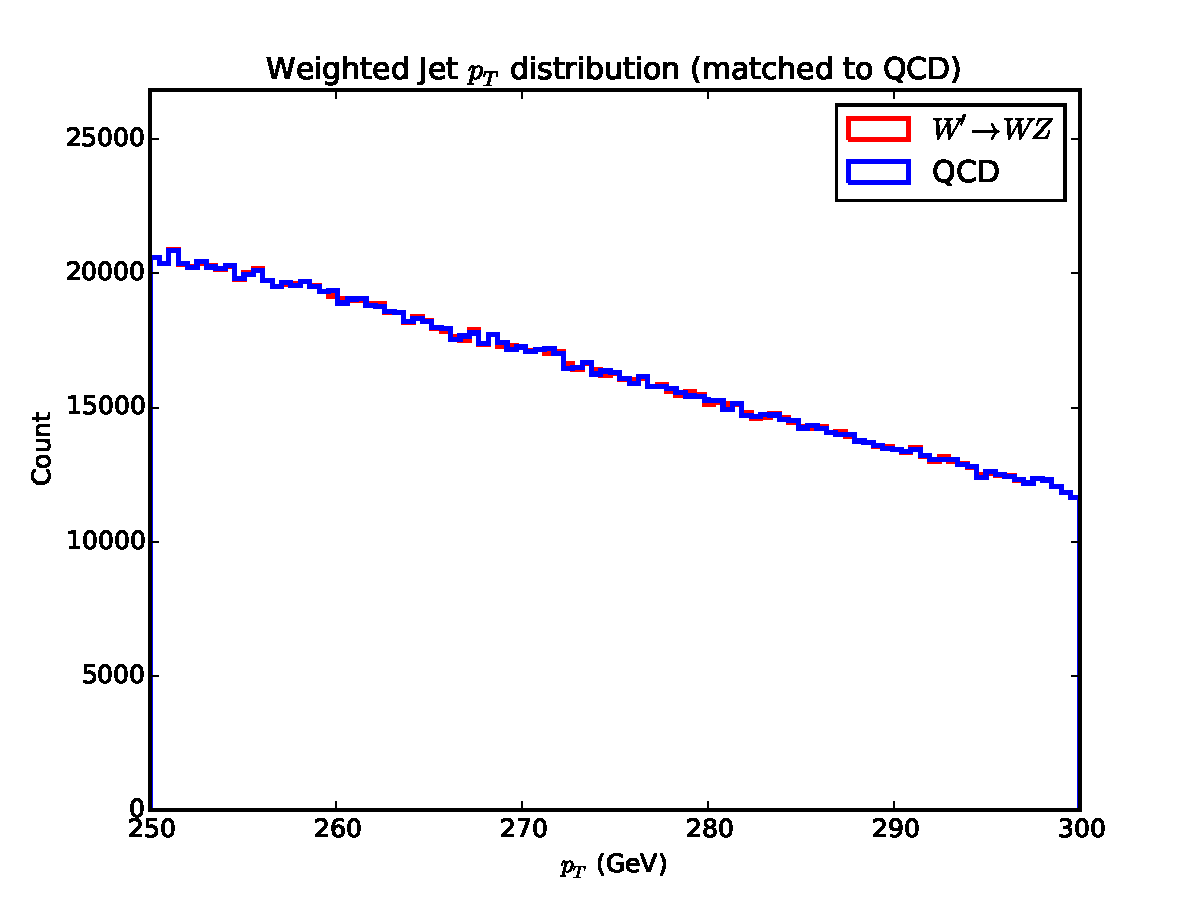
\includegraphics[width=0.5\textwidth]{figures/weighted-pt-distribution[250-300].pdf}
      }
      \caption{ Jets originating from the $W'\rightarrow WZ$ decay are re-weighted such that their $p_T$ spectrum matches that of QCD jets\label{fig:pt} }
    \end{center}
\end{figure}


\begin{figure}[bt]
  \begin{center}
  
  
      \subfloat[Weighted jet mass distribution \label{subfig:weighted_mass}]{
        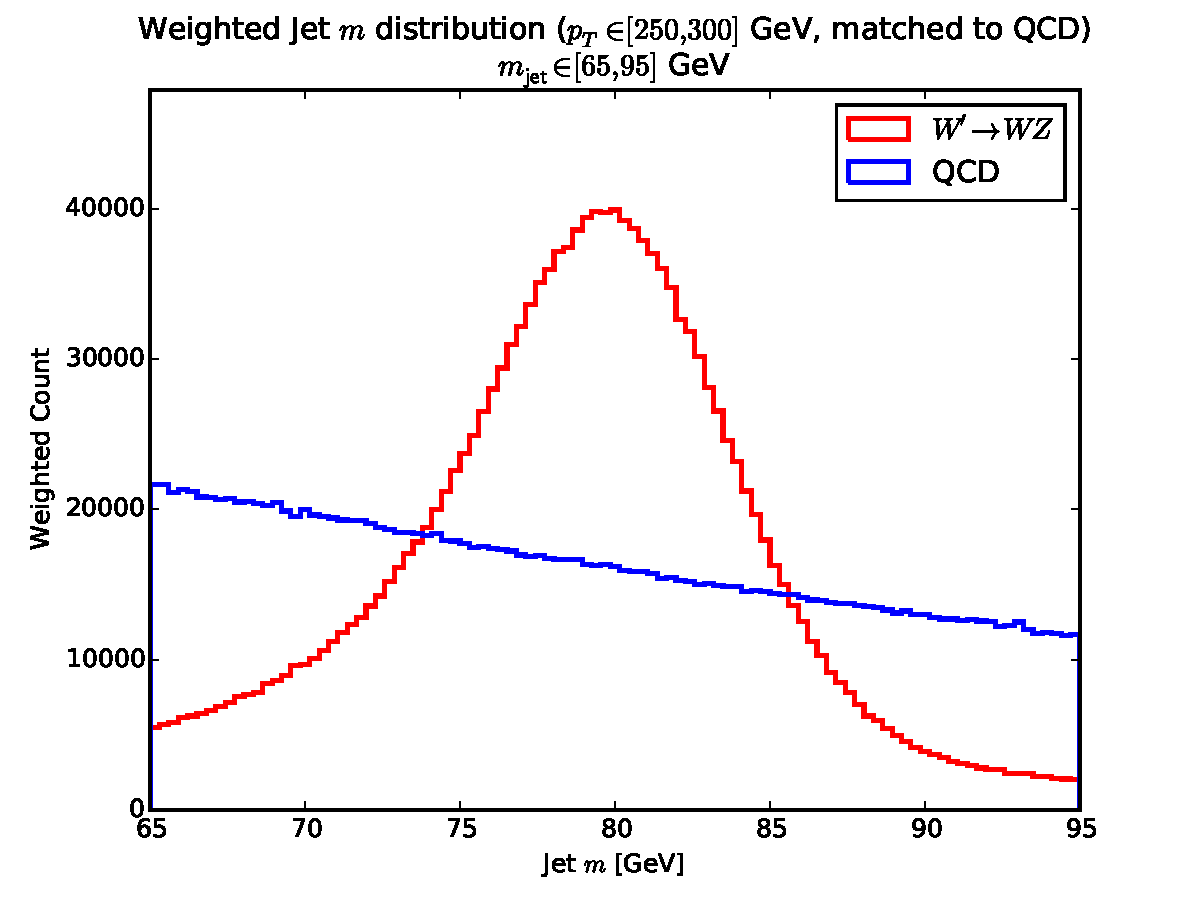
\includegraphics[width=0.5\textwidth]{figures/weighted-mass-distribution[250-300].pdf}
      }
      \subfloat[Weighted $\tau_{21}$ distribution \label{subfig:weighted_nsj}]{
        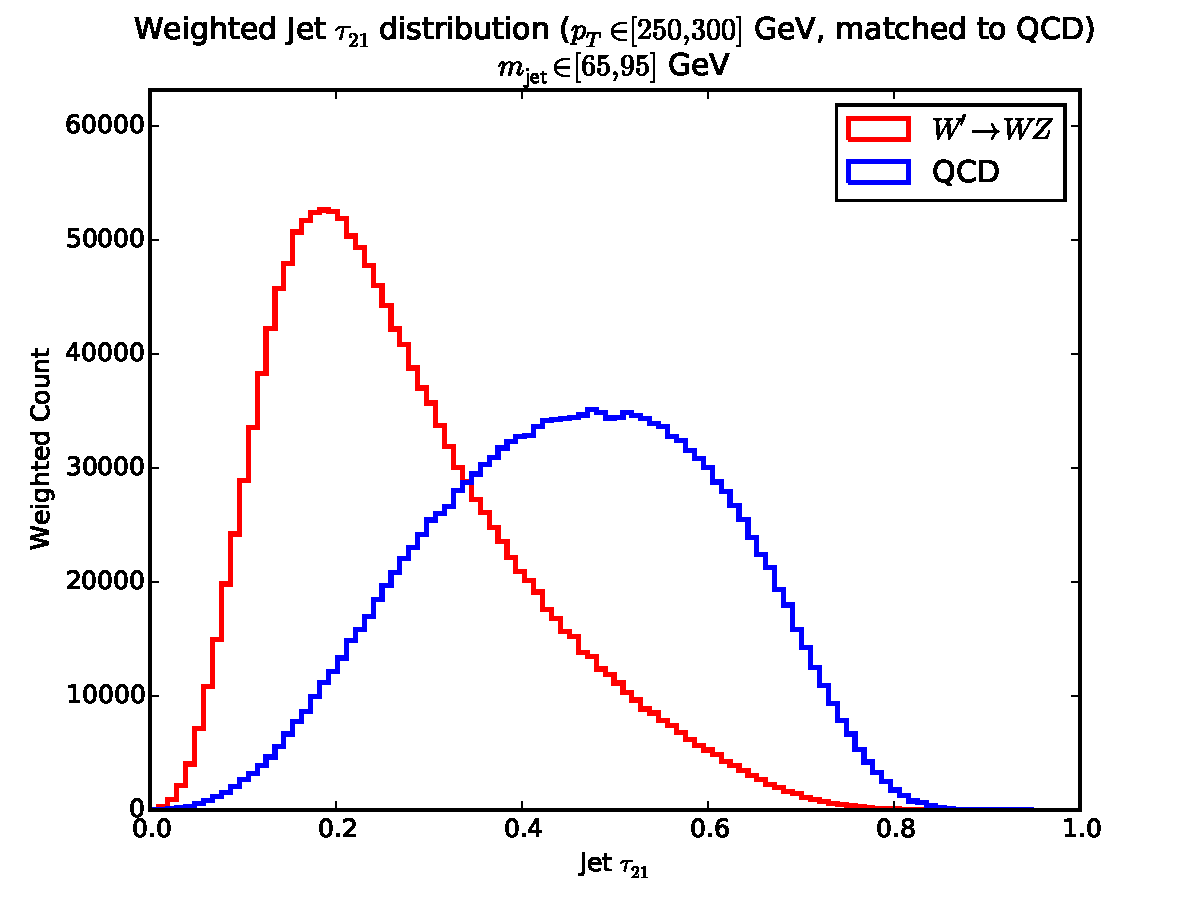
\includegraphics[width=0.5\textwidth]{figures/weighted-tau21-distribution[250-300].pdf}
      }
      \caption{Weighted mass (left) and $n$-subjettiness (right) of samples, with $W'\rightarrow WZ$ decays in red and QCD jets in blue.\label{fig:mass_nsj_spectrum} }
    \end{center}
\end{figure}  



\begin{figure}[bt]
  \begin{center}
  
      \subfloat[Average weighted $W'\rightarrow WZ$ image \label{subfig:weighted_sig}]{
        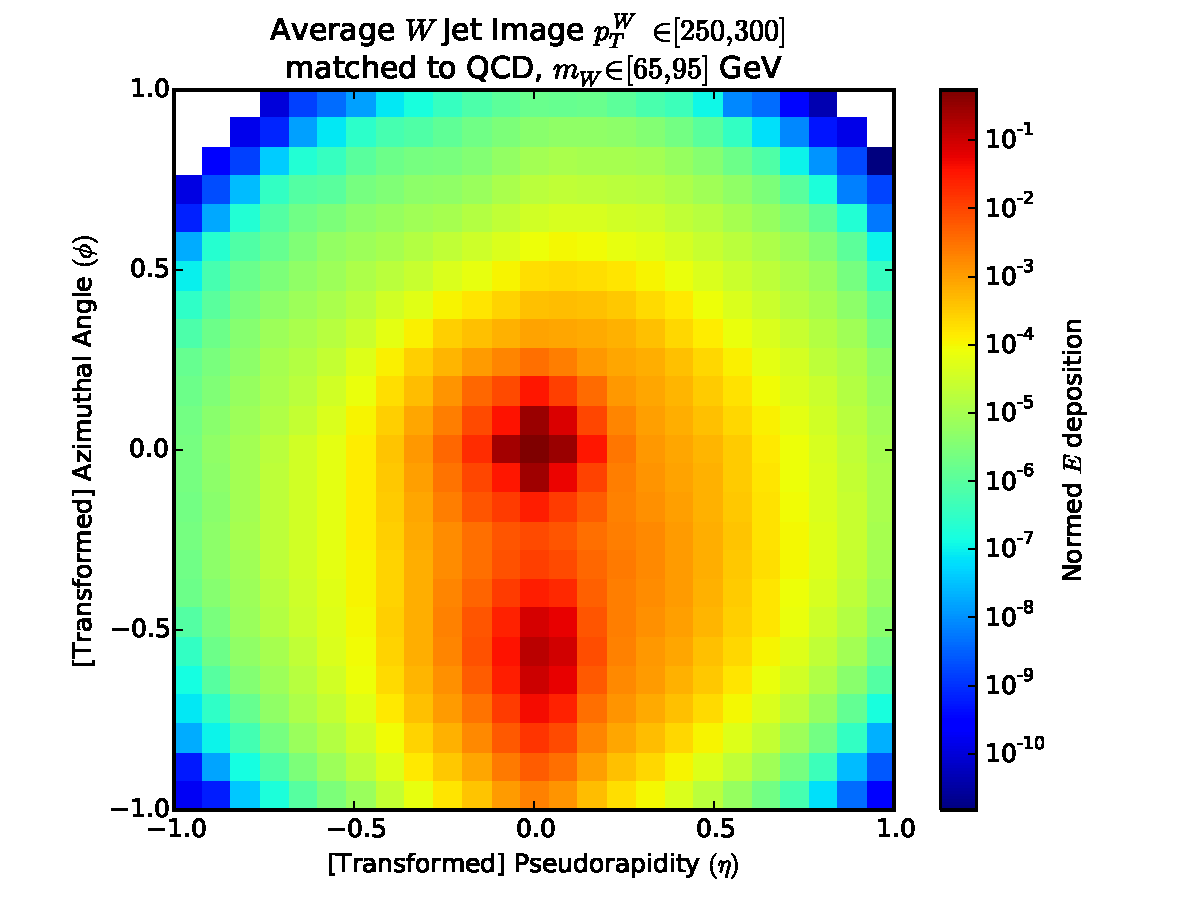
\includegraphics[width=0.5\textwidth]{figures/sig-im.pdf}
      }
      \subfloat[Average weighted QCD image \label{subfig:weighted_bkg}]{
        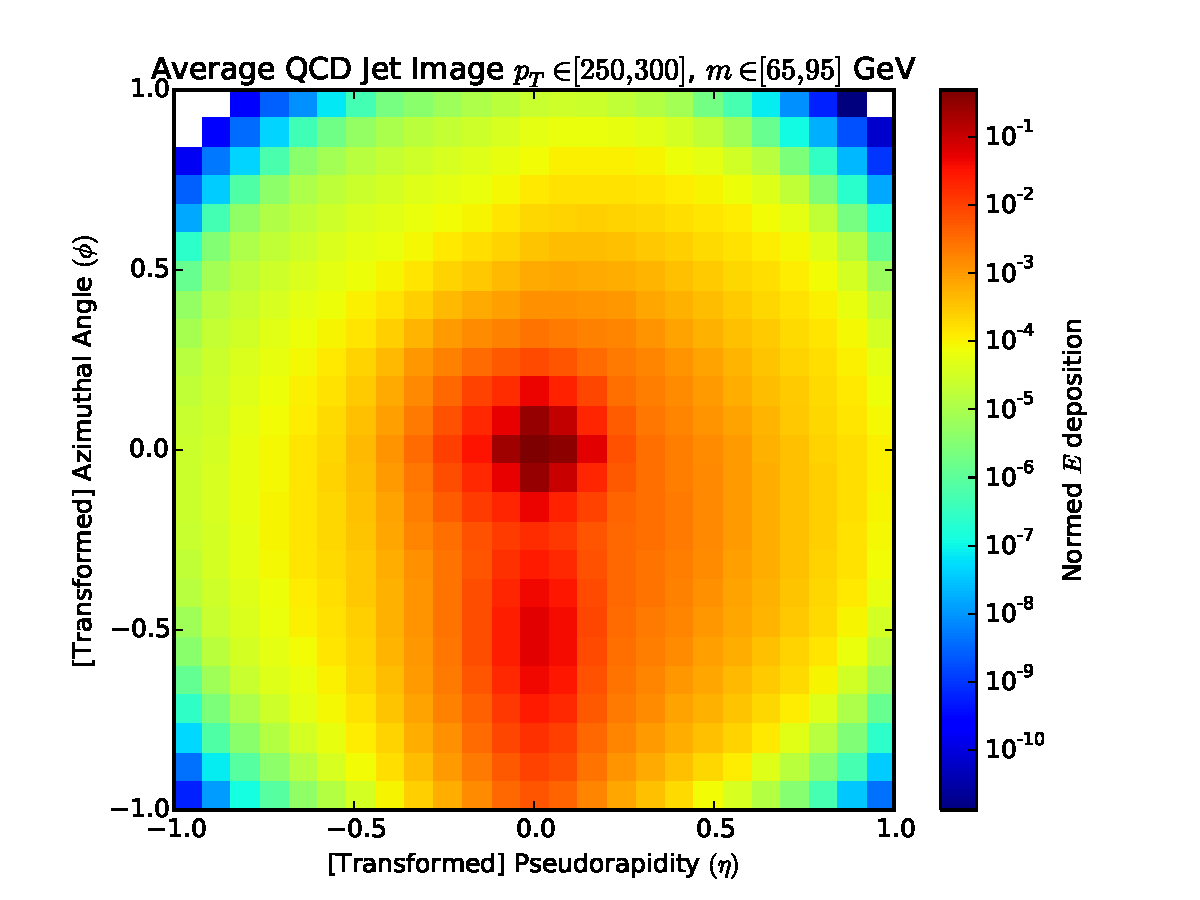
\includegraphics[width=0.5\textwidth]{figures/bkg-im.pdf}
      }
      \caption{Weighted $W'\rightarrow WZ$ (left) and QCD (right) average jet-image
      \label{fig:meanImages} }
    \end{center}
\end{figure}  



\section{Figure of Merit} % (fold)
\label{sec:figure_of_merit}

As is commonly done in High Energy Physics, we eschew the commonly chosen metric of basic accuracy in favor of the Receiver Operating characteristic. This is because we must examine the entire spectrum of trade-off between Type-I and Type-II error, as many applications in physics will choose different points along the trade-off curve. We use a slight modification of the traditional ROC. For any discriminating variable, let $c$ be a threshold on the likelihood ratio on that variable, and let $w$ be the vector of weights over the entire evaluation sample. We define the \emph{rejection} of such a threshold is defined as 
$$
    \rho(c) = \frac{1}{\text{FPR}(c, w)},
$$
where $\text{FPR}(c, w)$ is the weighted false positive rate for using $c$ as a threshold.

We define the \emph{efficiency} of $c$ as 
$$
    \varepsilon(c) = \text{TPR}(c, w),
$$
where $\text{TPR}(c, w)$ is the weighted false positive rate for using $c$ as a threshold. We then evaluate our algorithms using the area under the line generated by $\{(\varepsilon(c), \rho(c)) : \varepsilon(c)\in [0.2, 0.8]\}$. We say that an classifier is \emph{strictly} more performant if the ROC curve is above a baseline for all efficiencies.

% section figure_of_merit (end)


\section{Deep Learning}

Since it's first usage by it's current name~\cite{hinton06}, Deep Learning has taken on many forms and seen success in a variety of fields that have traditionally utilized human-engineered features to create classifiers and apply out-of-the-box machine learning algorithms. In particular, the field of Computer Vision has changed drastically. Since the 2012 ILSVRC winning entry by Alex Krizhevsky and the University of Toronto group ~\cite{alexnet}, Deep Learning -- in particular Convolutional Neural Networks -- have taken over vision-based machine learning, consistently showing human and recently super-human levels performance on key baseline datasets. The increasingly widespread availability of GPUs and associated numerical frameworks has made the time intensive estimation procedures associated with deep neural networks more feasible, and has allowed the size of models for image tasks to grow exponentially. For example, the Google team's contribution to ILSVRC 2014 -- the GoogLeNet~\cite{googlenet} -- consisted of 22 layers of convolutional black boxes called ``Inception Units'', and set the benchmarks both for accuracy and speed of a model on such a large scale. 

As it relates to our work, do not investigate large network architectures, rather we focus on  understanding what information and higher level representations a convolutional neural network will learn in the context of High Energy Physics. We let our knowledge of physics guide our investigations into visualization, understanding, and demystification of deep representations for physics. We shed light inside the black-box of deep learning in the context of object identification in HEP.


\section{Network Architecture}

%An in-depth examination of architectures via trial and error is left  future 

We begin with the notion that the discretization procedure outlined in Section \ref{sec:simulation} produces $25\times 25$ ``energy-scale'' images in one channel -- a High Energy Physics analogue of a grayscale image. We note that the images we work with are \emph{sparse} -- roughly 12\% of pixels are active on average. Future work can build on efficient techniques for exploiting the sparse nature of these images -- i.e., memoized convolutions. However, since speed is not our driving force in this work, we utilized convolution implementations defined for dense inputs.

\subsubsection{Architectural Selection} % (fold)
\label{ssub:architectural_selection}
We utilize a very simple convolutional architecture for our studies, consisting of two sequential \texttt{[Conv + Max-Pool + Dropout]} units, followed by two fully connected, dense layers. Our architecture can be succinctly written as 

\begin{equation}
  \mathtt{[Dropout \rightarrow Conv \rightarrow ReLU \rightarrow MaxPool] * 2 \rightarrow [Dropout \rightarrow FC \rightarrow ReLU] * 2 \rightarrow Sigmoid}.
\end{equation}

After early experiments with the standard $3\times 3$ kernel size, we discovered no improvement over a more basic MaxOut \cite{maxout:goodfellow} feedforward network. After further investigation into larger convolutional kernel size, we discovered that larger-than-normal kernels work well on our application. Though not common in the Deep Learning community, we hypothesize that this larger kernel size is helpful when dealing with sparse structures in the input images. In Table~\ref{tab:kernelsize}, we show the optimal kernel size of $11\times11$ while considering the metric outlined in Section~\ref{sec:figure_of_merit}.

\begin{table}[h!]
  \centering
  \begin{tabular}{r|c}
    \bfseries Kernel size & \bfseries AUC \\ 
    \hline
    $(3 \times 3)$ Conv & 14.770 \\
    \hline
    $(4 \times 4)$ Conv & 12.452 \\
    \hline
    $(5 \times 5)$ Conv & 11.061 \\
    \hline
    $(7 \times 7)$ Conv & 13.308 \\
    \hline
    $(9 \times 9)$ Conv & 17.291 \\
    \hline
    $(11 \times 11)$ Conv & 20.286 \\
    \hline
    $(15 \times 15)$ Conv & 18.140 \\
  \end{tabular}
  \caption{First layer convolution size vs. performance}
  \label{tab:kernelsize}
\end{table}
% table

We follow up the first layer of convolutions with Rectified Linear Unit activations, then utilize $(2, 2)$ max-pooling to downsample. We then use $(4\times 4)$ convolutions in the second convolutional unit + $(2, 2)$ max-pooling, and connect to 64 units then one final output.
% subsubsection architectural_selection (end)

\subsubsection{Implementation and Training} % (fold)
\label{ssub:implementation_and_training}


Event generation and simulation was conducted on the SLAC \texttt{atlint} cluster. All Deep Learning experiments were conducted in Python with the Keras~\cite{Keras} Deep Learning library on the Stanford Institute for Computational and Mathematical Engineering GPU cluster, utilizing NVIDIA C2070 graphics cards. 

We used 30 million training and 30 million testing samples, and trained networks using both the Adam~\cite{DBLP:journals/corr/KingmaB14} algorithm and Stochastic Gradient Descent with Nesterov Momentum~\cite{Nesterov:1983wy}. We found that SGD+Nesterov outperformed Adam, and thus is used in all following facts and figures.

% subsubsection implementation_and_training (end)


\section{Studies} % (fold)
\label{sec:studies}

To begin understanding what a deep network can learn about jet topology, we choose a finite region of phase space, and standardize our comparisons. In an effort to define a standard way that physics object identification using machine learning should be conducted, we exactly define our procedure for comparisons. In particular, we restrict our studies to $250$ GeV $\leq p_T \leq 300$ GeV, and confine ourselves to a $65$ GeV $\leq m \leq 95$ GeV mass window, wholly containing the peak of the $W$. 

We construct a scaffolded and multi-approach series of methodologies for understanding, visualizing, and validating neural networks within HEP.

\subsection{Coarse Studies} % (fold)
\label{sub:coarse_studies}

To a first order, the first desirable characteristic is a simple performance improvement over the standard physics-driven variables for discrimination. In particular, we compare our network to $n$-subjettiness~\cite{nsub} and the jet mass. We henceforth refer to $n$-subjettiness as $\tau_{21}$ for our purposes, as $\tau_{2}/\tau_{1}$ is relevant for our classification problem.

In Figure~\ref{fig:combinedROC}, we illustrate the performance gains of a deep neural network over both $\tau_{21}$ and the 2D likelihood of $\tau_{21}$ and jet mass. 


\begin{figure}[!htbp]
  \centering
  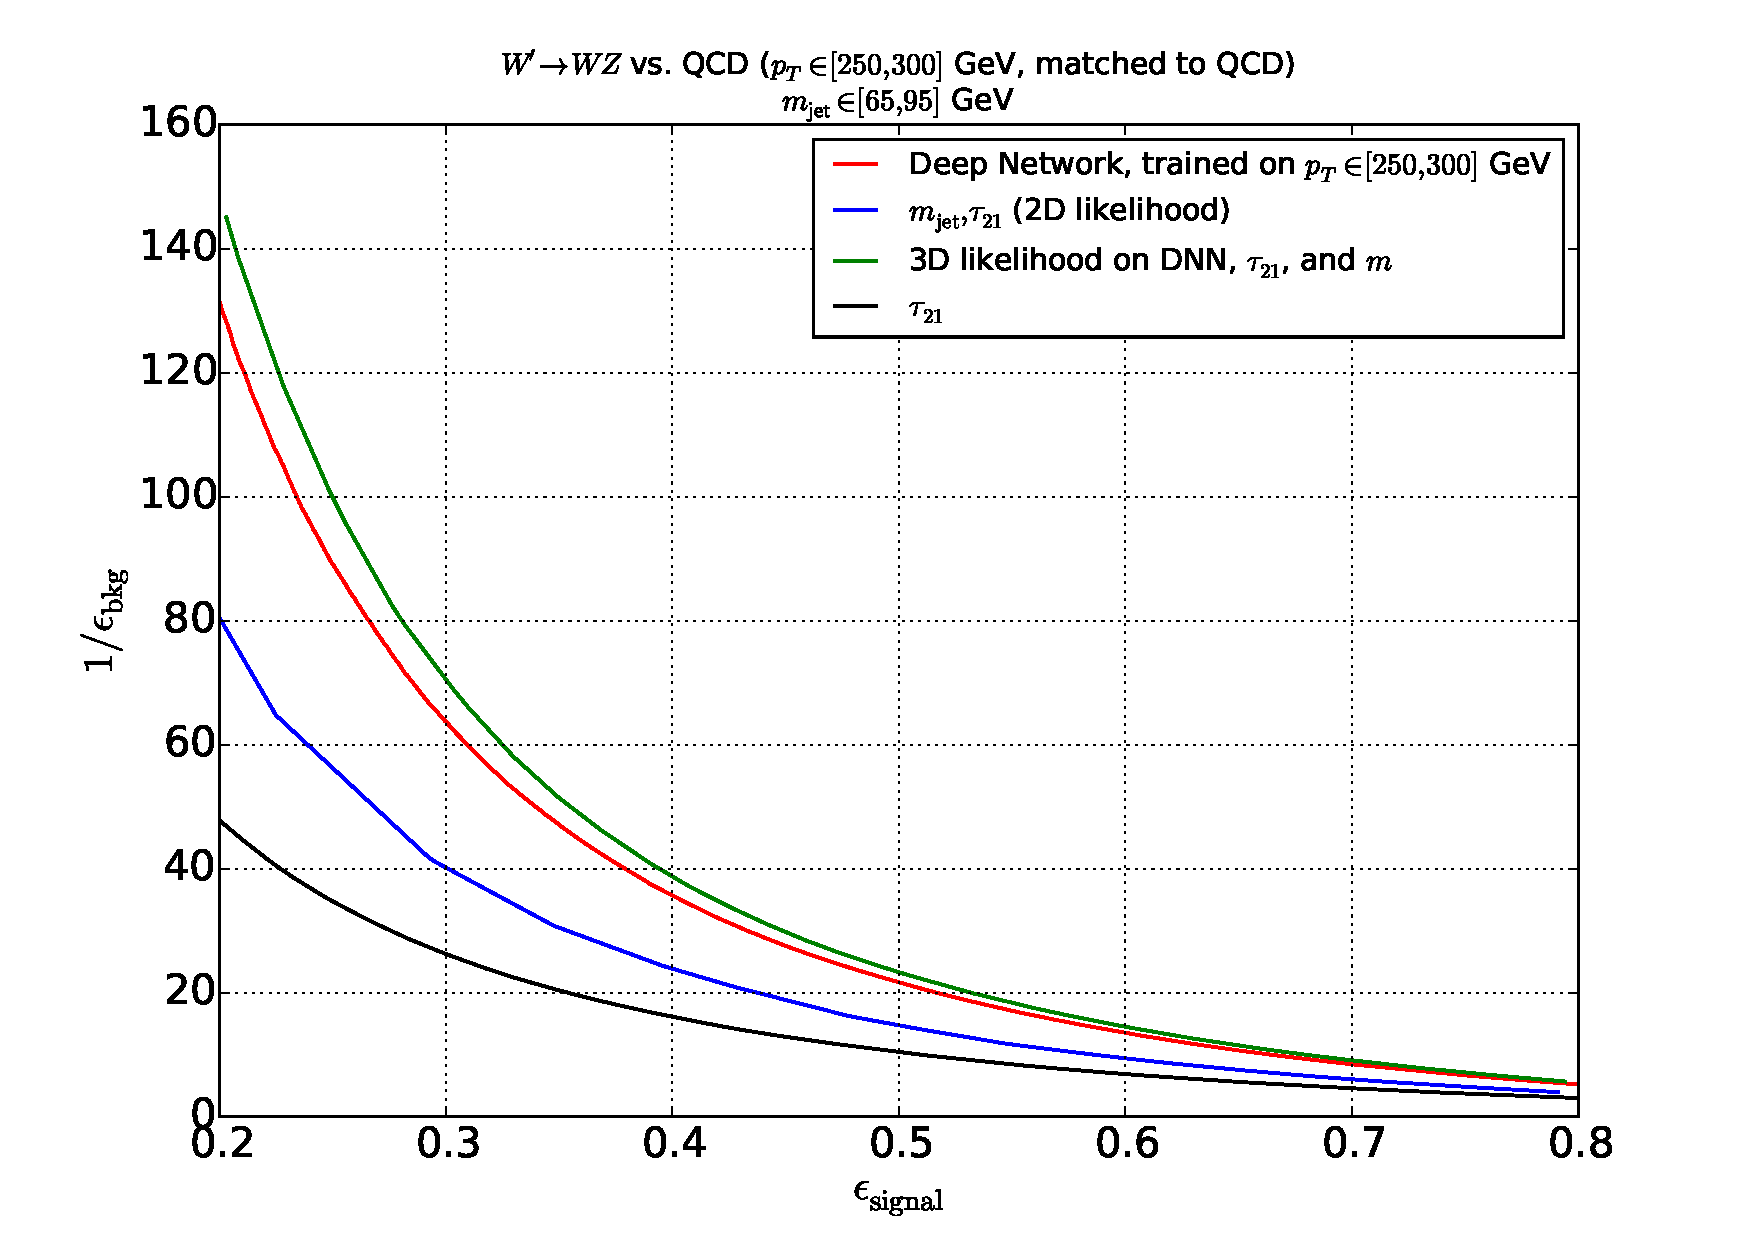
\includegraphics[width=0.95\textwidth]{figures/combined-roc.pdf}
  \caption{Receiver Operating Characteristic (ROC) over coarse sample}
  \label{fig:combinedROC}
\end{figure}

We also provide a comparison to a 3D likelihood constructed on $\tau_{21}$, jet mass, and the deep network output itself. We can gain a significant piece of insight from this. Note how in Figure~\ref{fig:combinedROC} we can see that the DNN represents a large gain on a physics-only likelihood. However, when we explicitly include the physics variable in a 3D likelihood, we see a small but definitively non-zero performance gain. This implies that the performance boost \emph{by definition} is getting its gain from something that is not \emph{fully} encapsulated in $\tau_{21}$ and jet mass. 

Though important on it's own, this figure of merit does little to help drive understanding in the context of HEP. Such an increase begs further questions -- what is this gain, and where does it come from? Why is the DNN able to pick up on this?



\subsubsection{Understanding what is learned} % (fold)
\label{ssub:understanding_what_is_learned}

% subsubsection understanding_what_is_learned (end)
In Figure~\ref{fig:convkernels}, we first examine the $11\times11$ convolutional filters in the first layer and look for structure. In

In order to understand what we learn, we first take a look \emph{inside} the deep network. 
\begin{figure}[bt]
  \begin{center}
      \subfloat[$(11\times11)$ convolutional kernels from first layer \label{subfig:filters}]{
        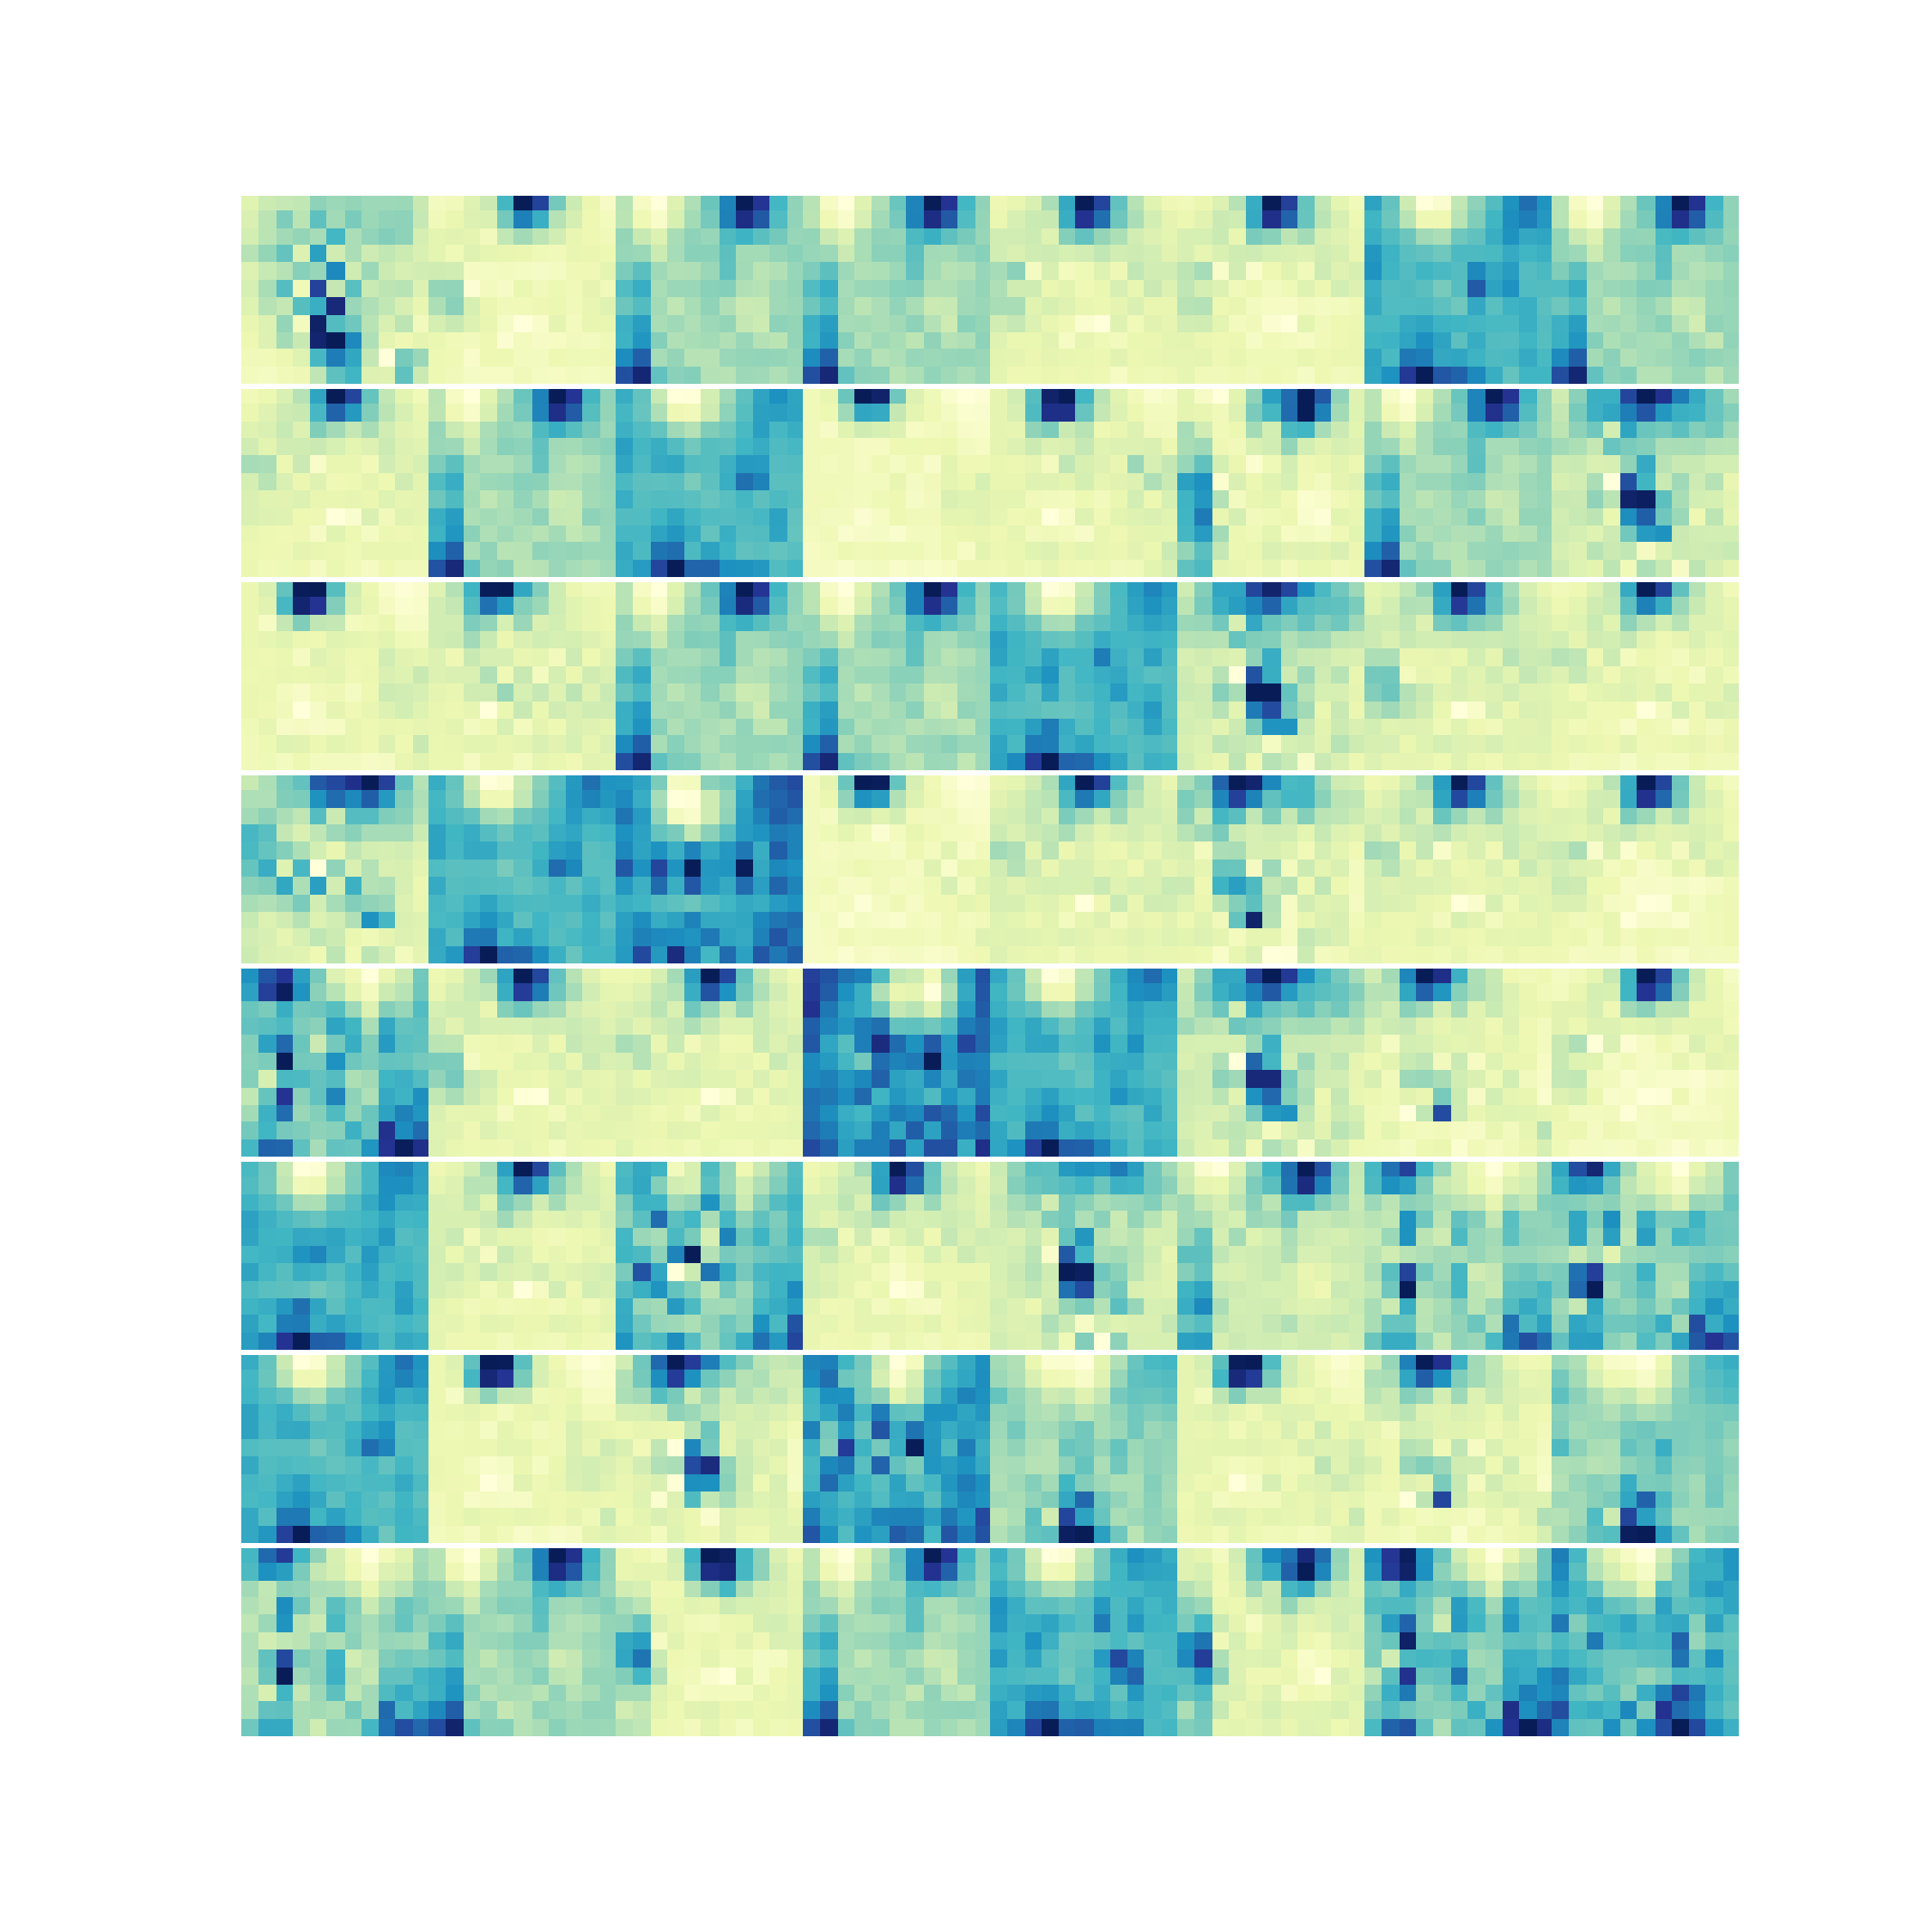
\includegraphics[width=0.5\textwidth]{figures/conv-filts.pdf}
      }
      \subfloat[Convolved Jet Image differences\label{subfig:convolvedfilters}]{
        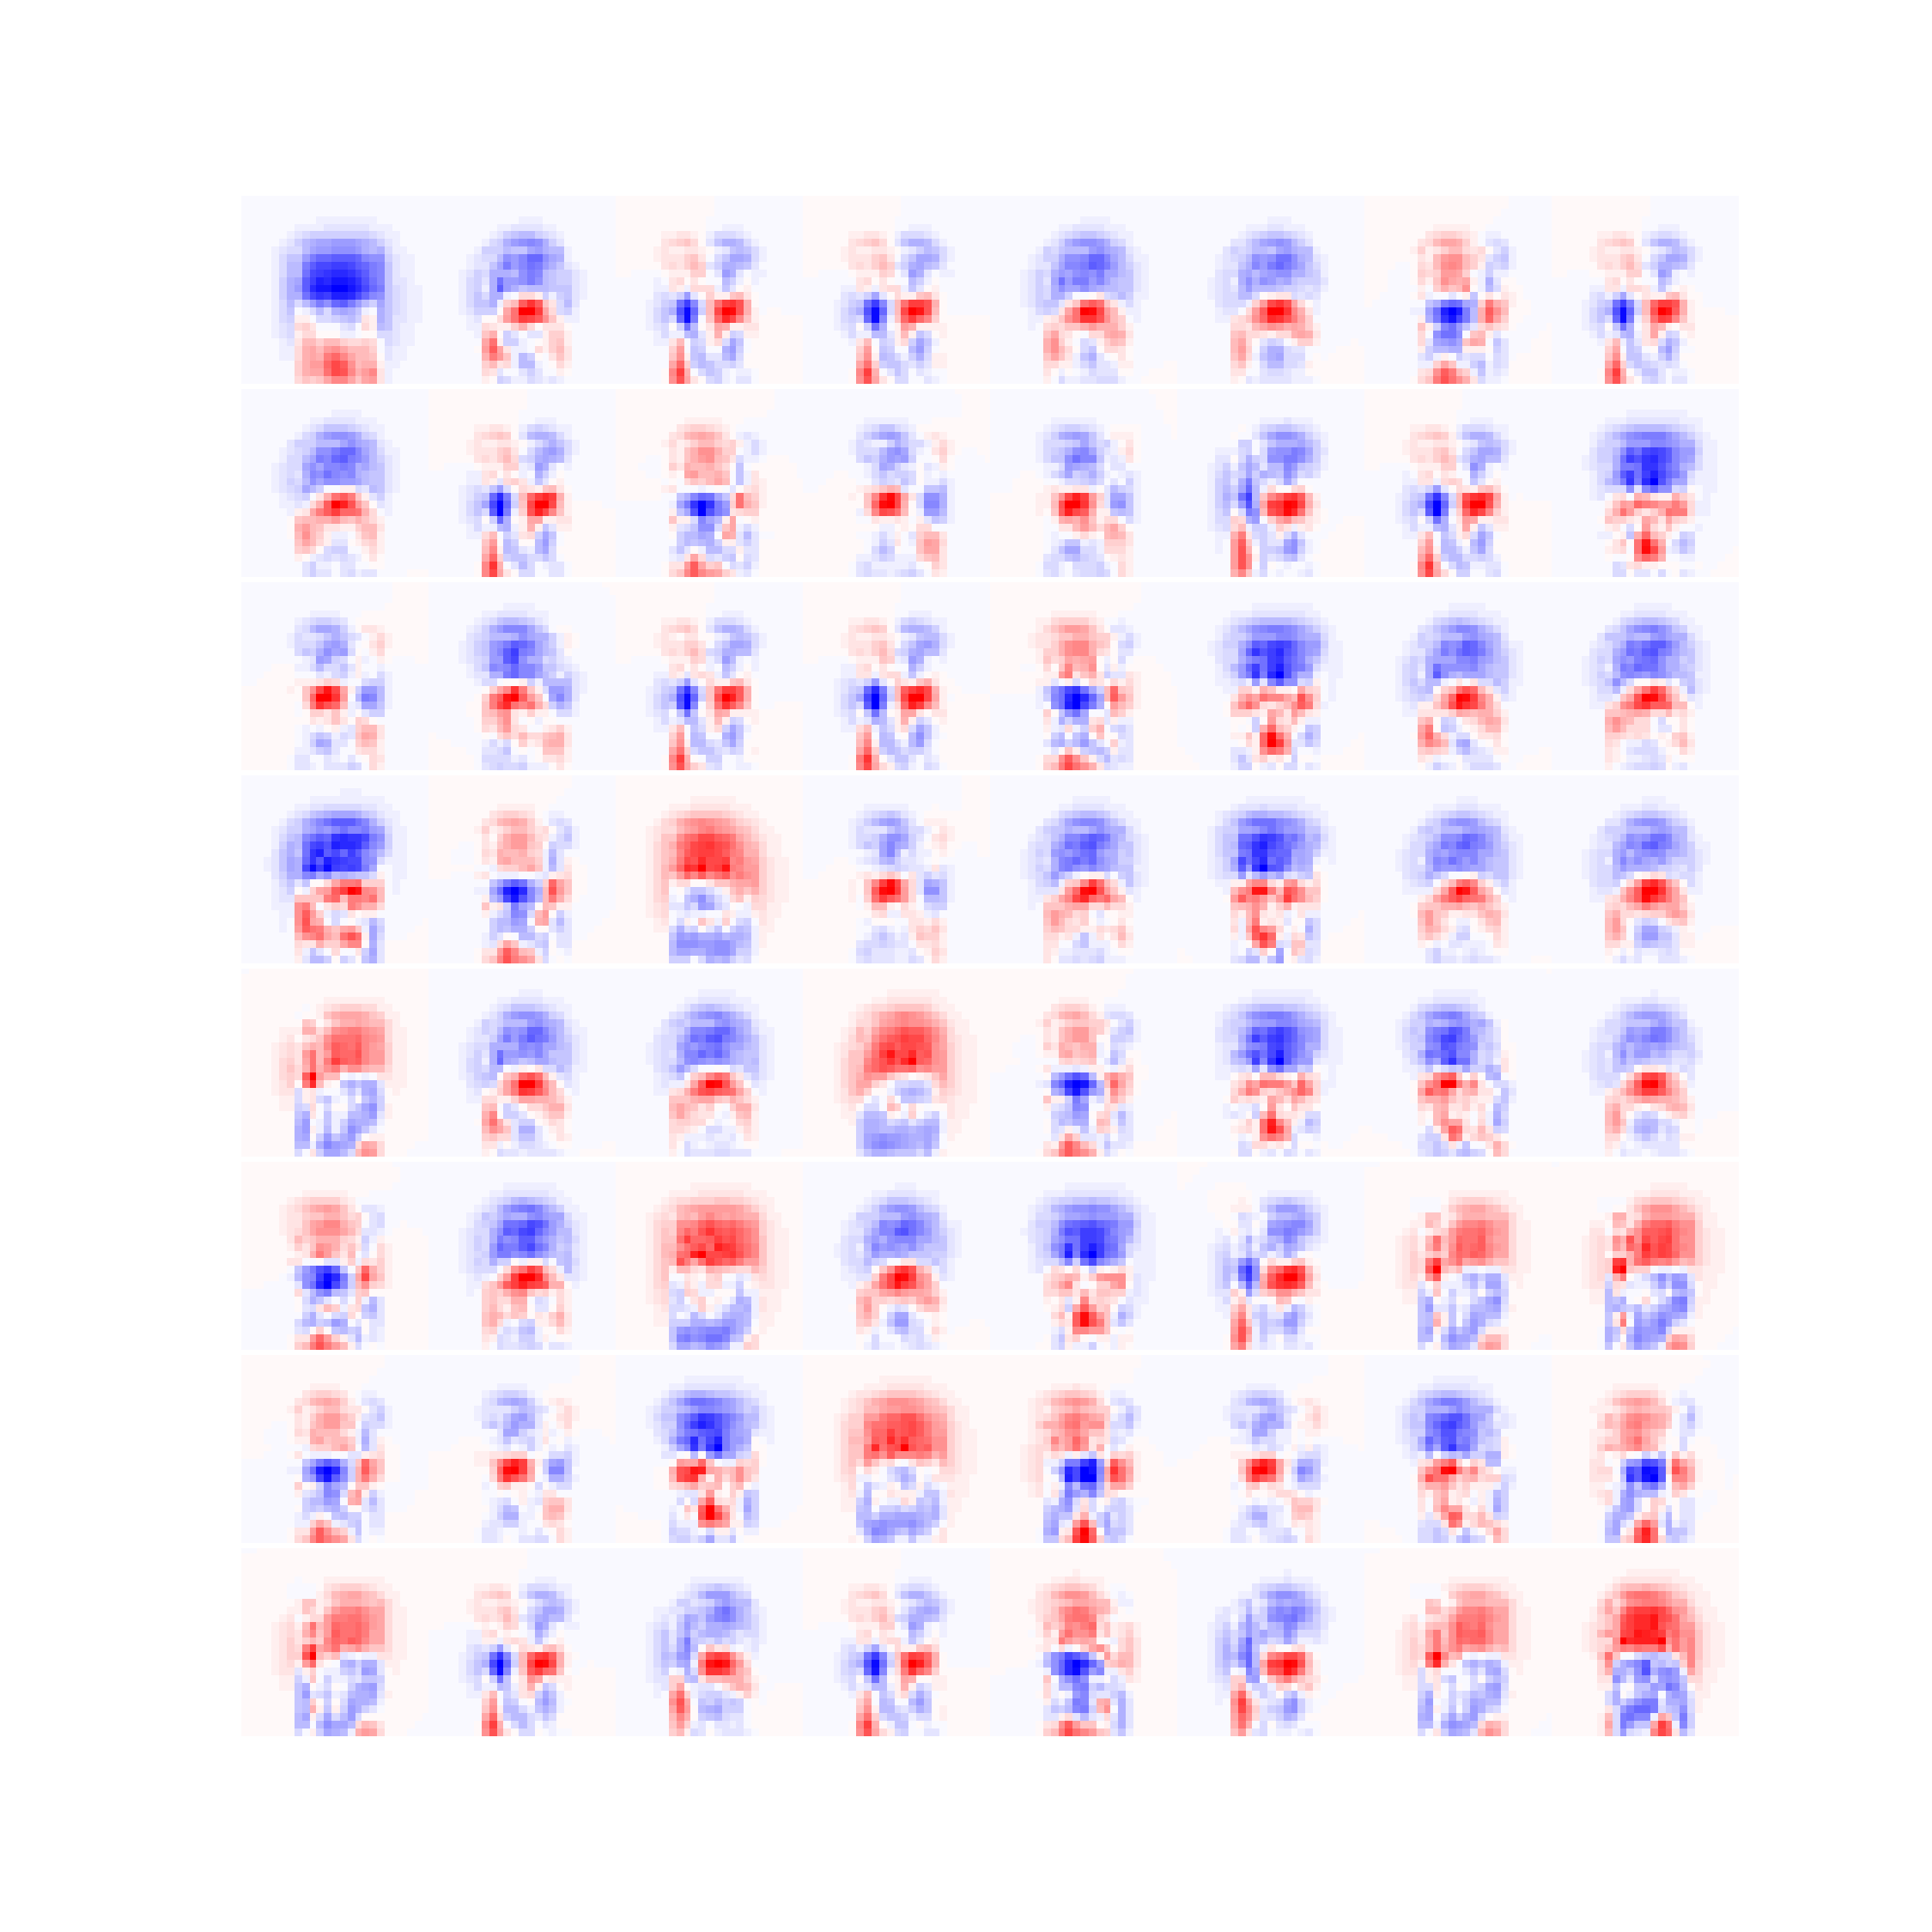
\includegraphics[width=0.5\textwidth]{figures/conv-diffs-global.pdf}
      }
      \caption{Convolutional Kernels (left), and convolved feature differences in jet images (right)}
      \label{fig:convkernels}

    \end{center}
\end{figure}



Blah... linear correlations with pixels





\subsubsection{Physics in Deep Representations} % (fold)
\label{ssub:physics_in_deep_representations}


\begin{figure}[!htbp]
  \centering
  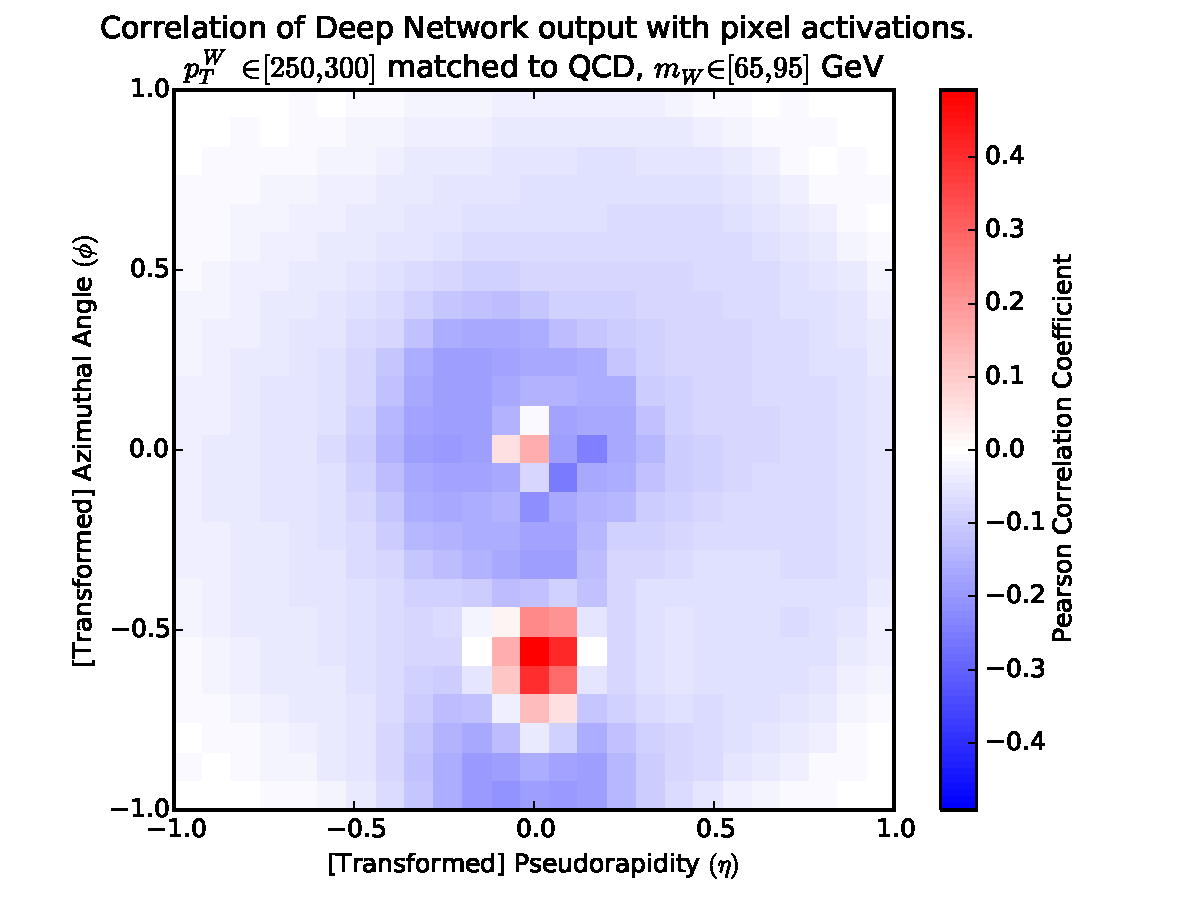
\includegraphics[width=0.95\textwidth]{figures/pixel-activations-corr.pdf}
  \caption{Per-pixel linear correlation with DNN output}
  \label{fig:corr}
\end{figure}


\begin{figure}[bt]
  \begin{center}
      \subfloat[Sculpted QCD $\Delta R$ distribution\label{fig:sculpteddR}]
      {
        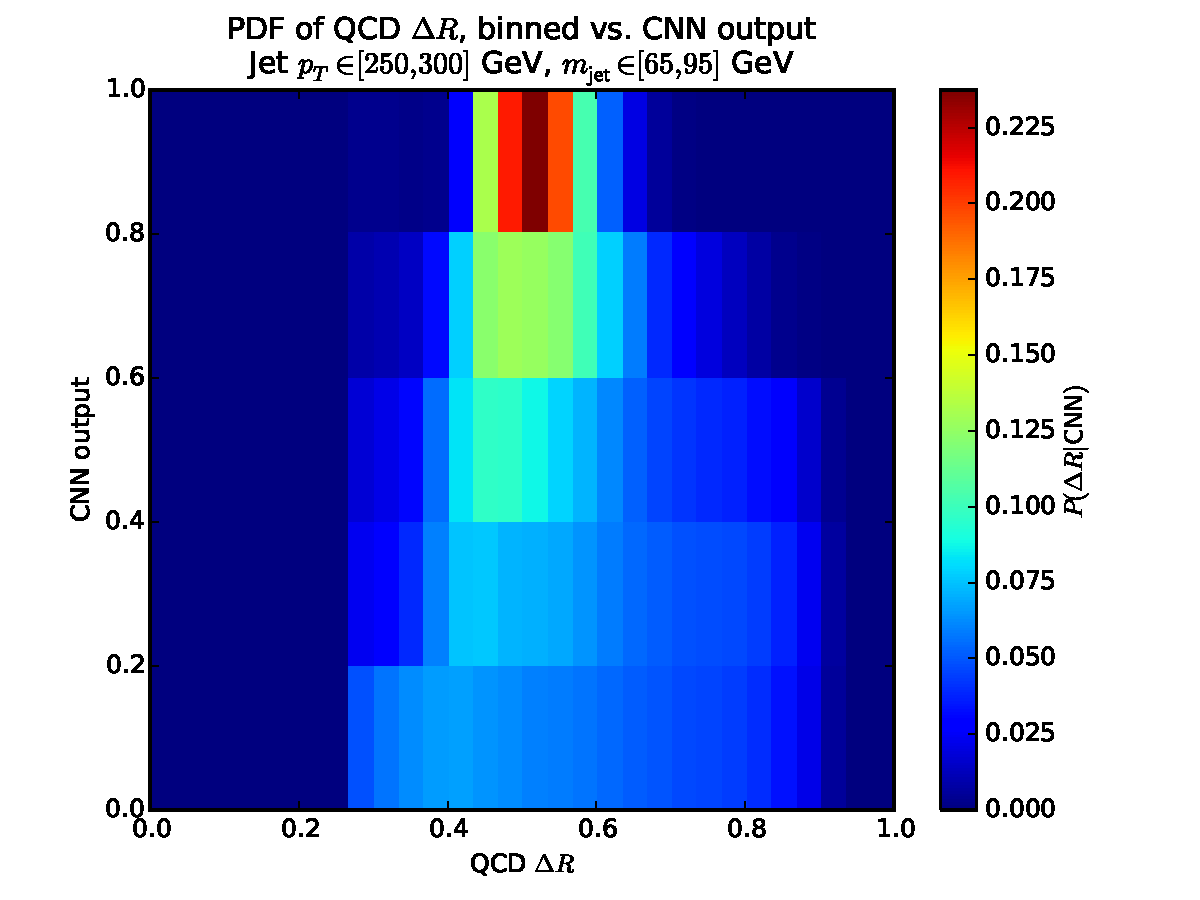
\includegraphics[width=0.5\textwidth]{figures/dR-dist-by-CNN.pdf}
      }
      \subfloat[Sculpted QCD $\tau_{21}$ distribution\label{fig:sculptednsj}]
      {
        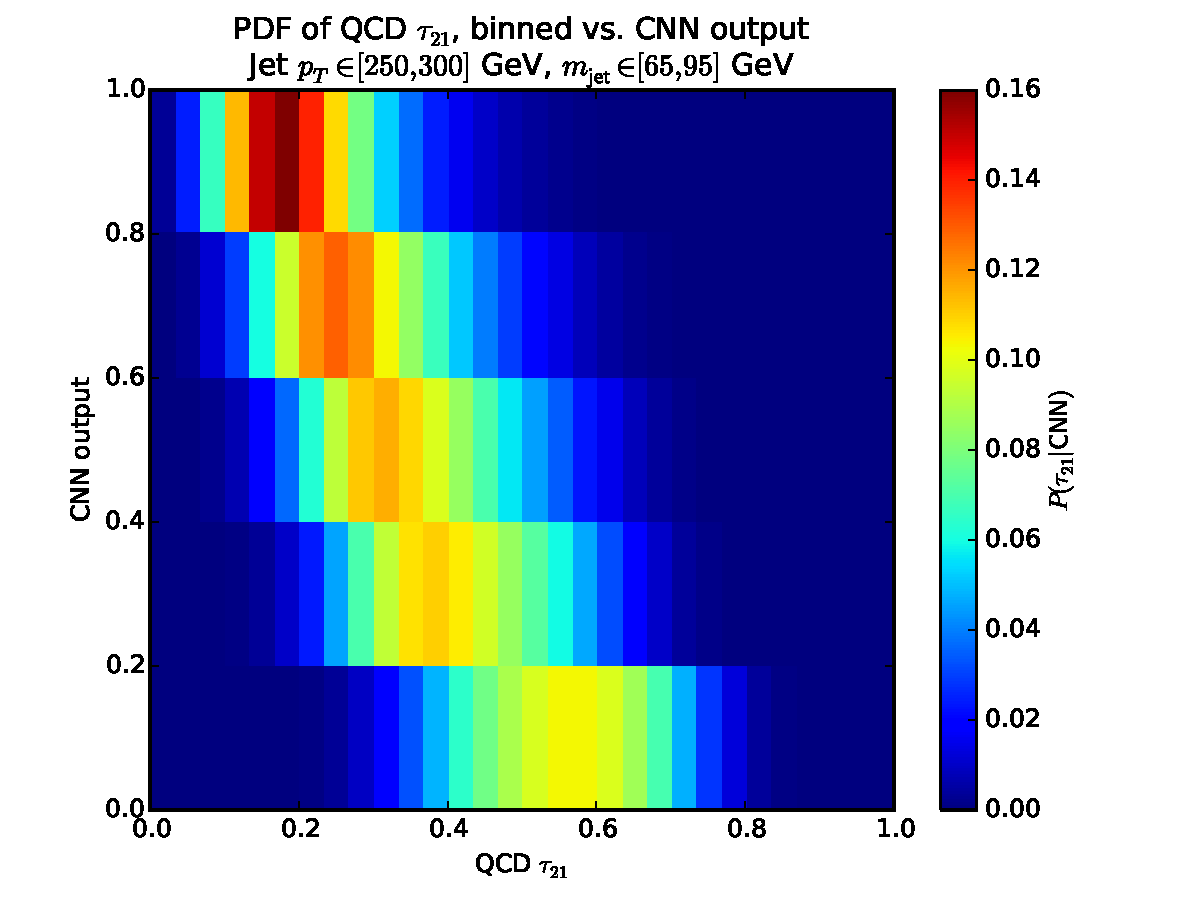
\includegraphics[width=0.5\textwidth]{figures/tau-dist-by-CNN.pdf}
      }
      \\
      \subfloat[Sculpted QCD mass distribution\label{fig:sculptedmass}]
      {
        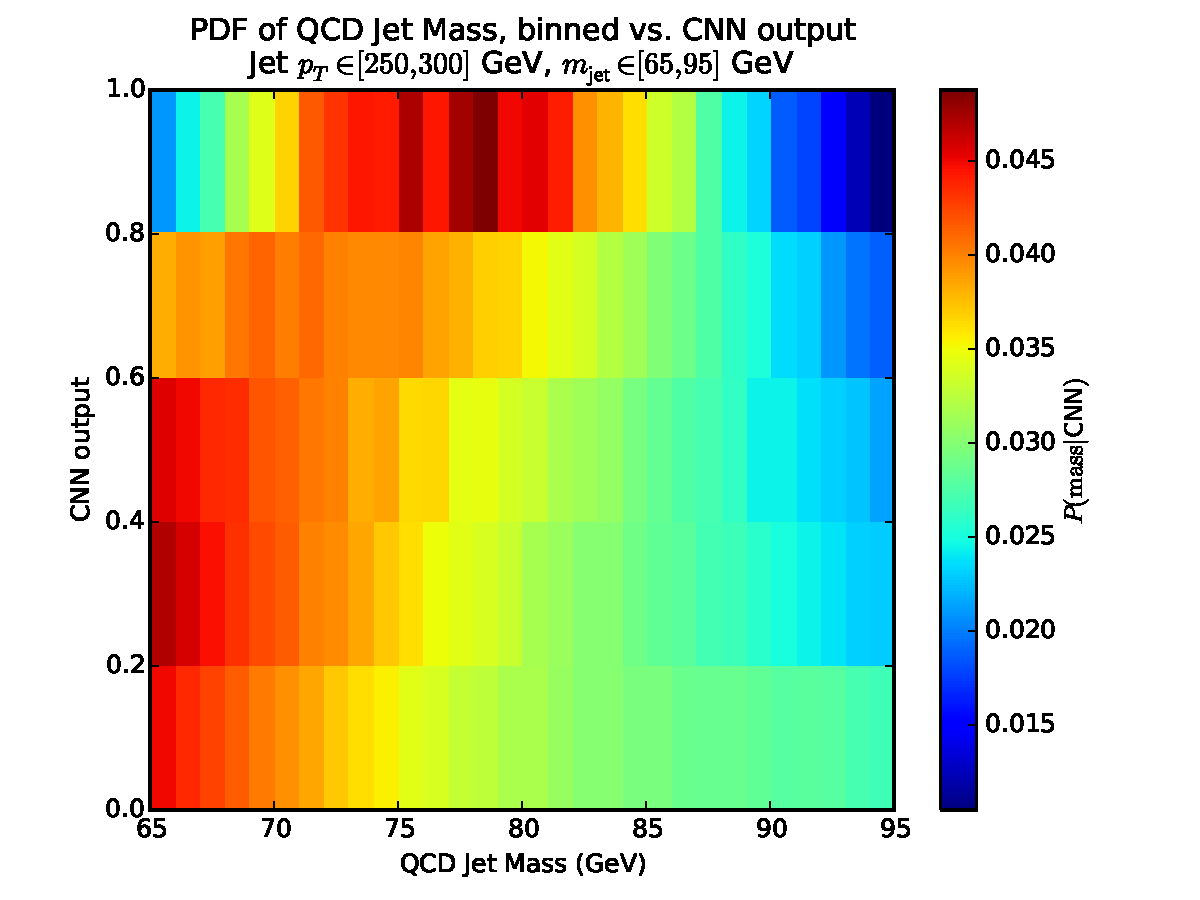
\includegraphics[width=0.5\textwidth]{figures/mass-dist-by-CNN.pdf}
      }

      \caption{Sculpted QCD distributions}
      \label{fig:qcdsculpt}

    \end{center}
\end{figure}





% subsubsection physics_in_deep_representations (end)

% subsection coarse_studies (end)

\subsection{Flat Hypercube Studies} % (fold)
\label{sub:flat_hypercube_studies}


Here, we see the ROC blah...

\begin{figure}[htbp]
  \centering
  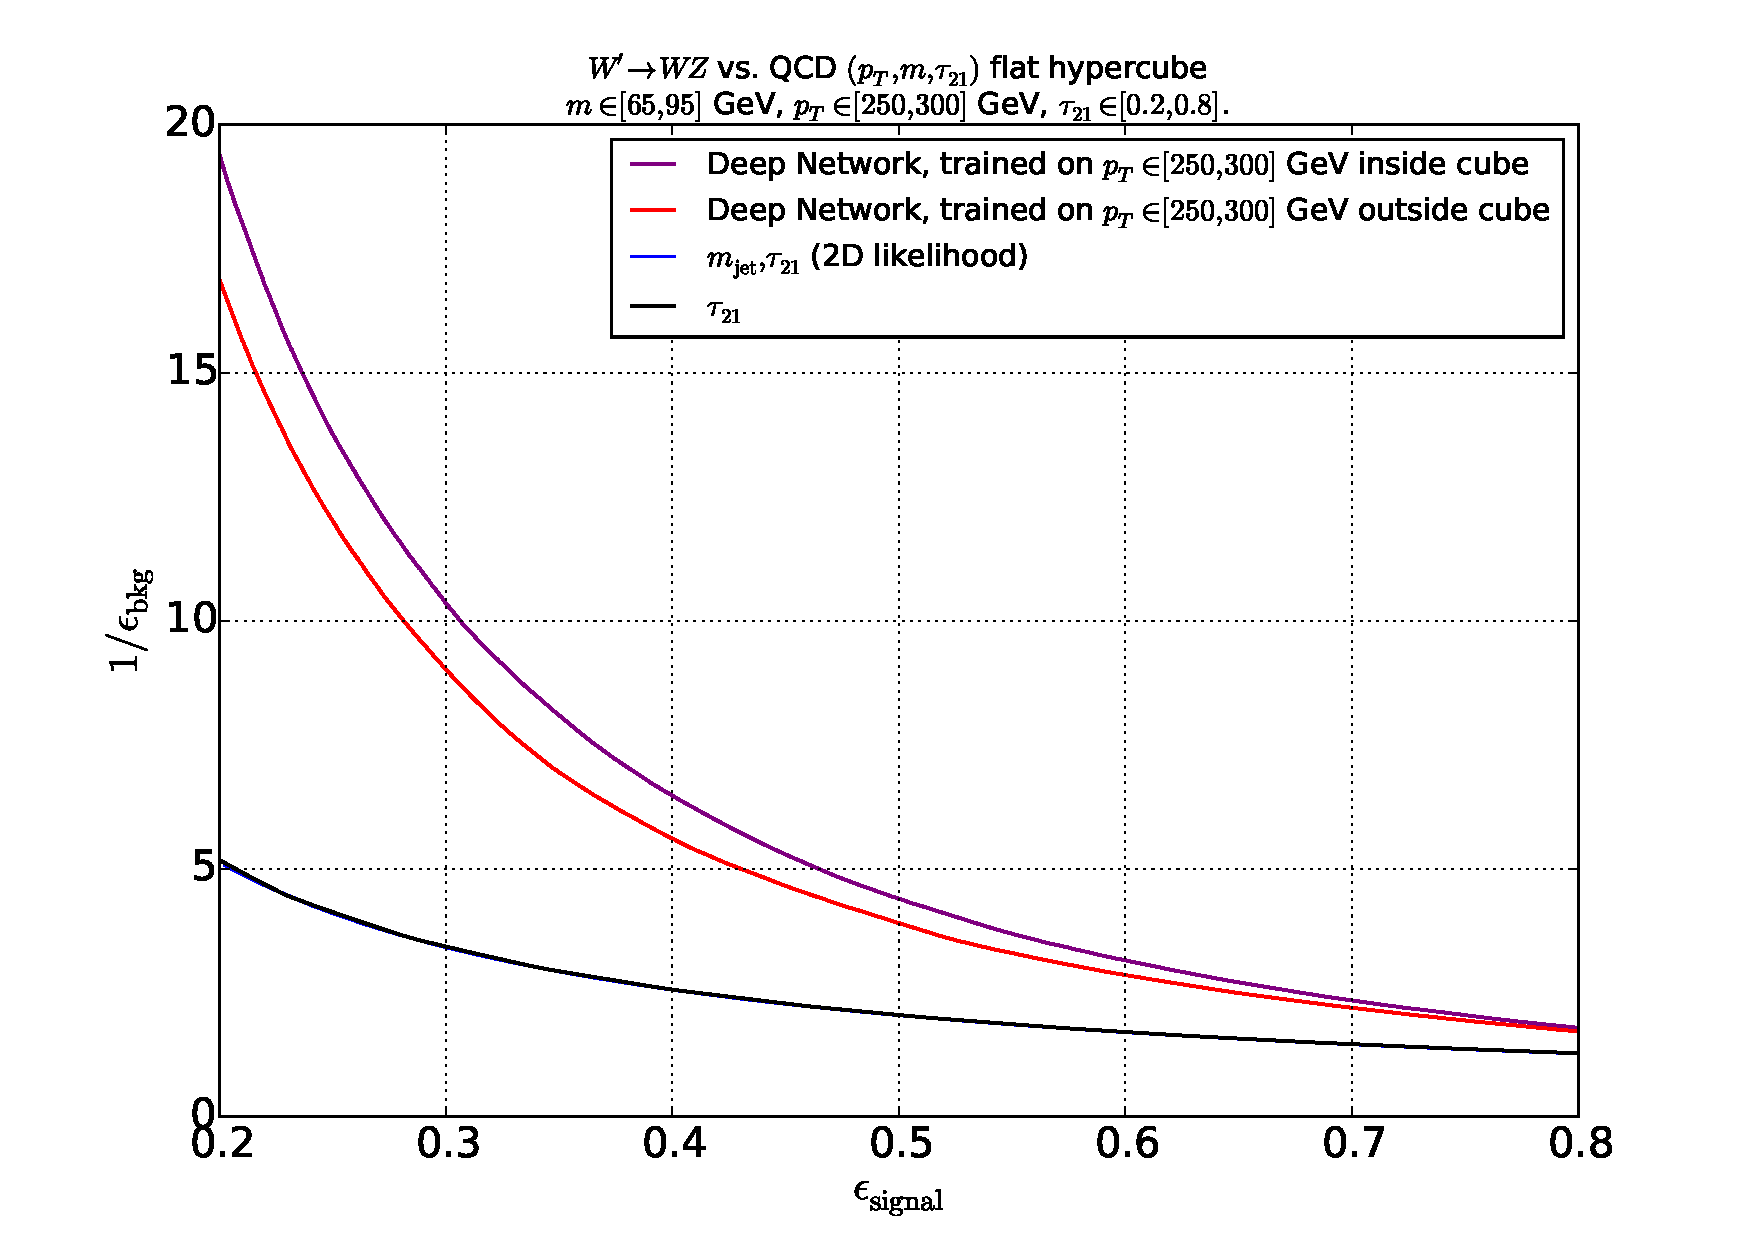
\includegraphics[width=0.95\textwidth]{figures/roc-cube-inside.pdf}
  \caption{ROC Curve for weigth-flattened hypercube, with $m\in[65, 95]\mathsf{GeV}$,  $p_T\in[250, 300]\mathsf{GeV}$, and  $\tau_{21}\in[0.2, 0.8]$}
  \label{fig:rocCube}
\end{figure}

% subsection flat_hypercube_studies (end)



\subsection{Small Window Studies} % (fold)
\label{sub:small_window_studies}


\begin{figure}[bt]
  \begin{center}
  
      \subfloat[Average $W'\rightarrow WZ$ image \label{subfig:sig_window}]{
        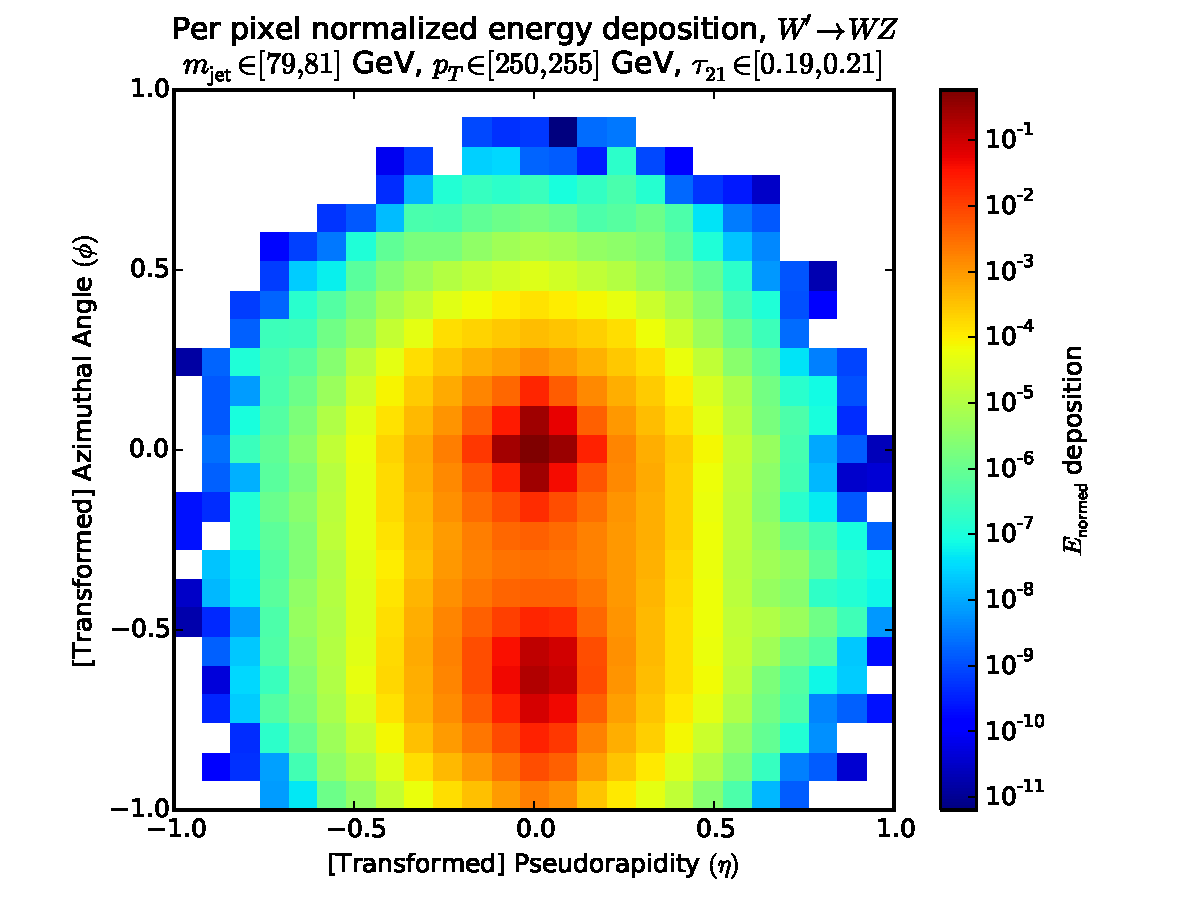
\includegraphics[width=0.5\textwidth]{figures/avg-benwindow-sig.pdf}
      }
      \subfloat[Average QCD image \label{subfig:bkg_window}]{
        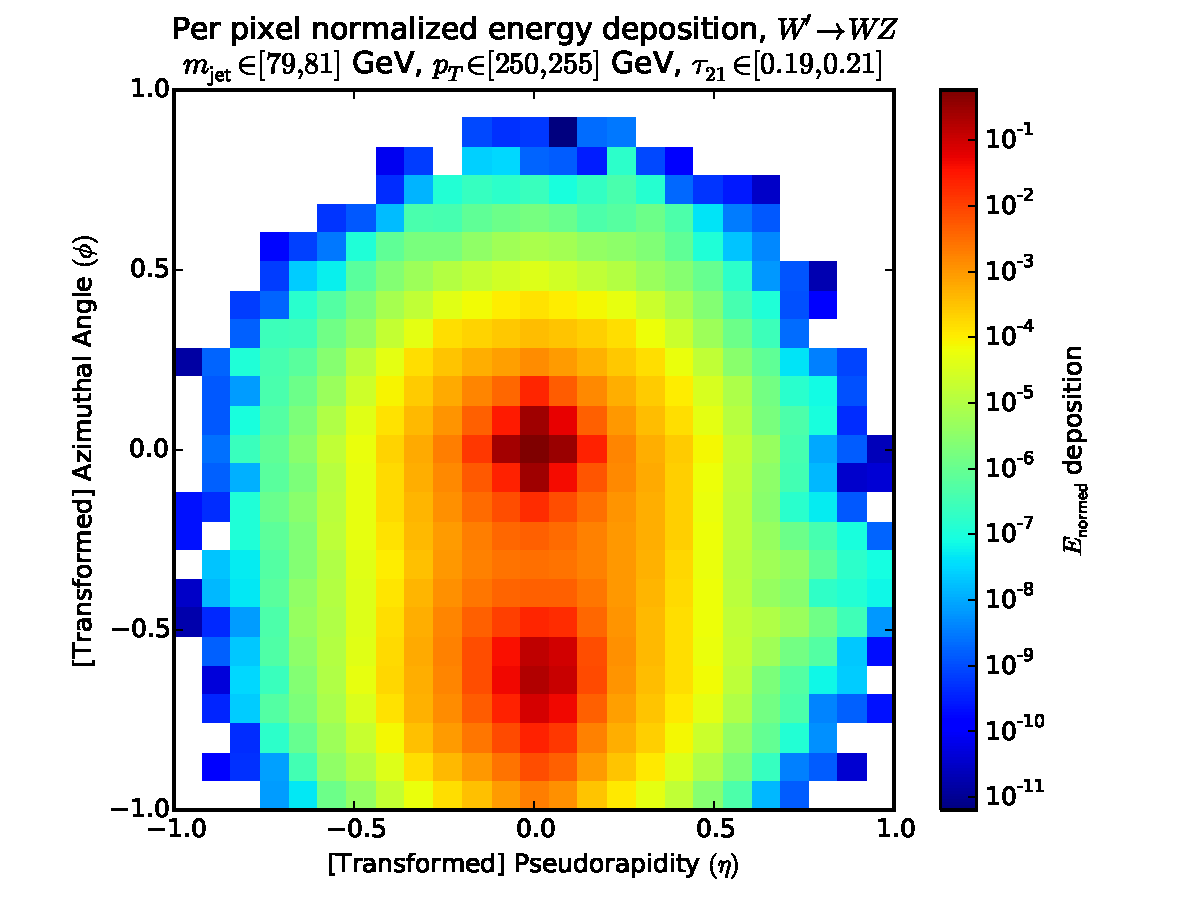
\includegraphics[width=0.5\textwidth]{figures/avg-benwindow-sig.pdf}
      } \\
      \subfloat[Average image difference \label{subfig:windowdiff}]{
        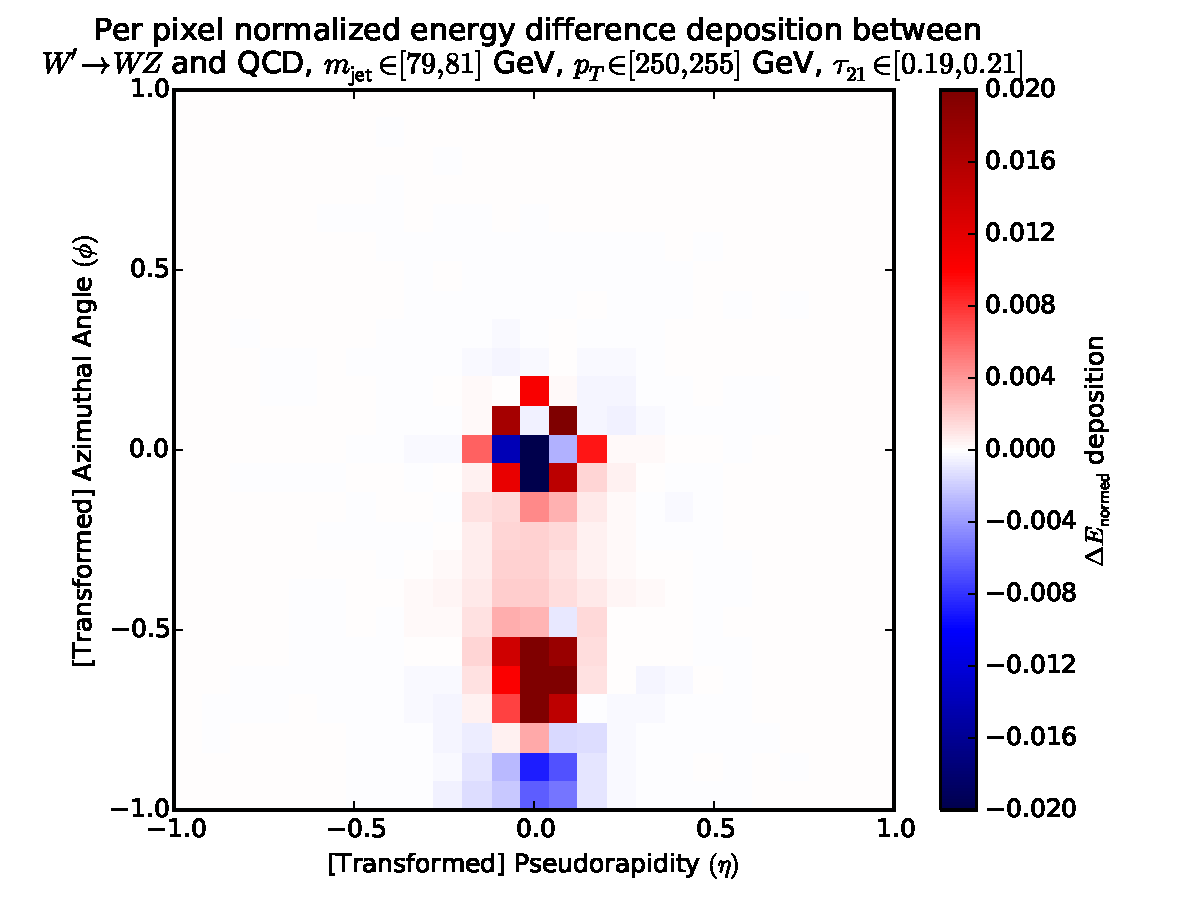
\includegraphics[width=0.5\textwidth]{figures/avg-benwindow-diff-clipped.pdf}
      }
      \caption{$W'\rightarrow WZ$ (left) and QCD (right) average jet-images, and Signal - Background image difference (bottom)
      \label{fig:meanImagesWindow} }
    \end{center}
\end{figure}  


Performance inside the window, use a Fisher Discriminant...

\begin{figure}[htbp]
  \centering
  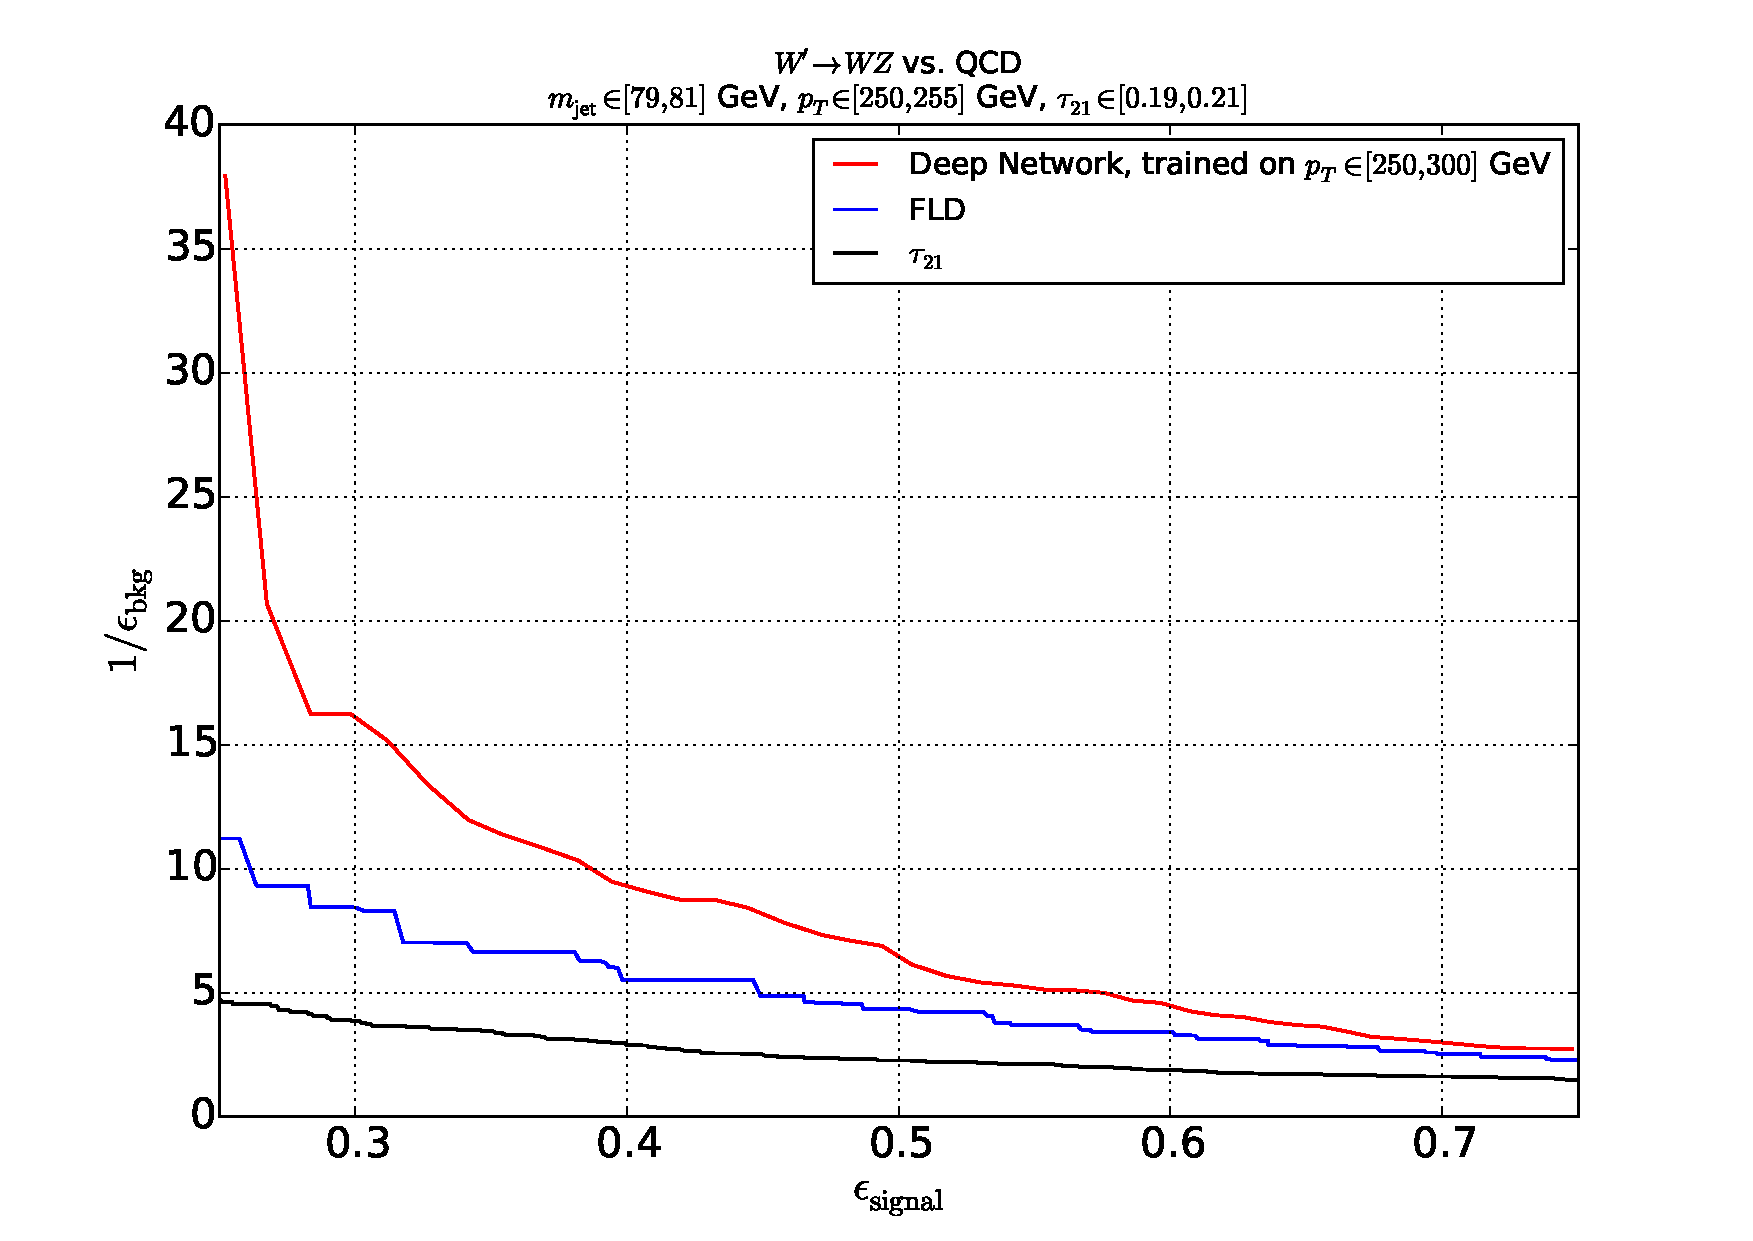
\includegraphics[width=0.95\textwidth]{figures/augwindow-roc.pdf}
  \caption{Receiver Operating Characteristic (ROC) over window sample}
  \label{fig:rocWindow}
\end{figure}

\subsubsection{Understanding what we learn} % (fold)
\label{ssub:understanding_what_we_learn}

\begin{figure}[htbp]
  \centering
  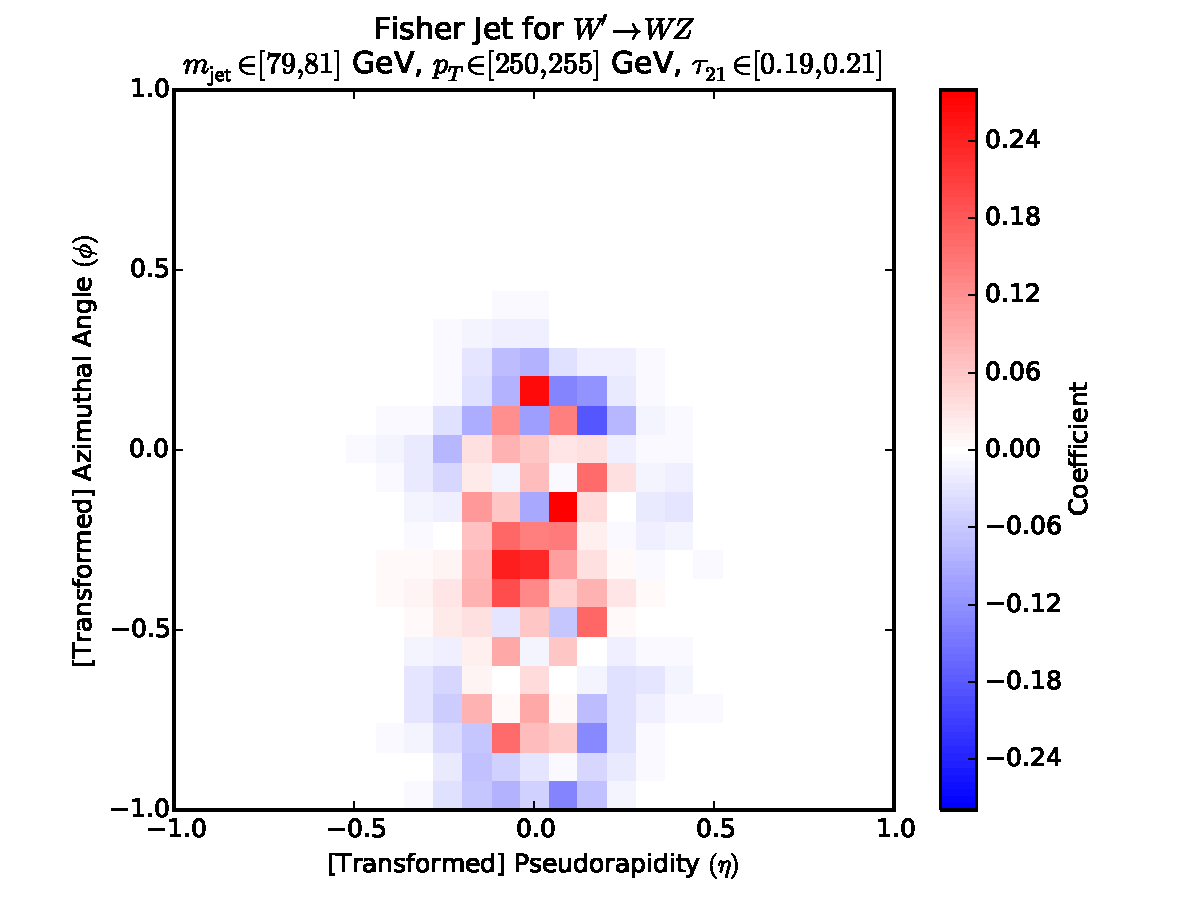
\includegraphics[width=0.65\textwidth]{figures/fld-benwindow.pdf}
  \caption{caption}
  \label{fig:fldWindow}
\end{figure}

\begin{figure}[htbp]
  \centering
  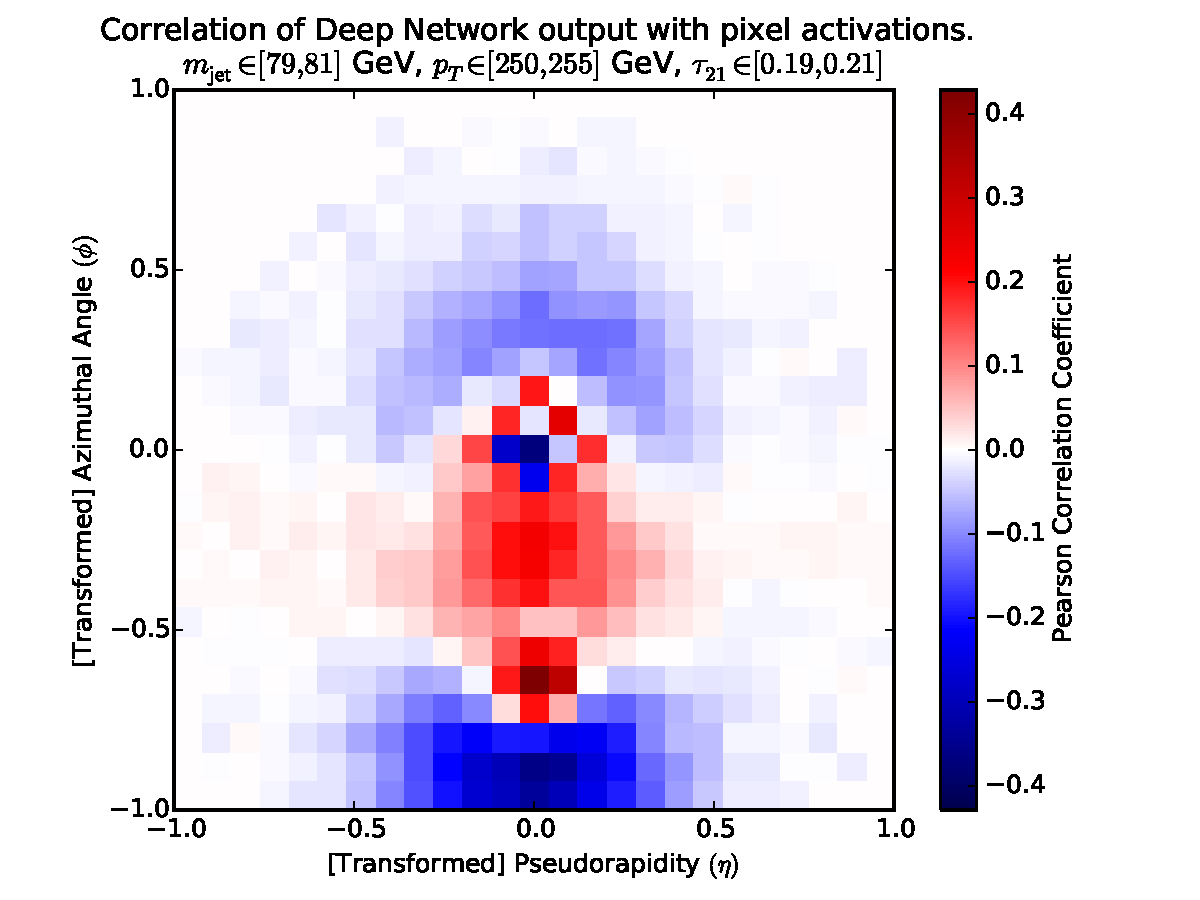
\includegraphics[width=0.65\textwidth]{figures/pixel-activations-corr-benwindow.pdf}
  \caption{caption}
  \label{fig:corrWindow}
\end{figure}


\begin{figure}[htbp]
  \centering
  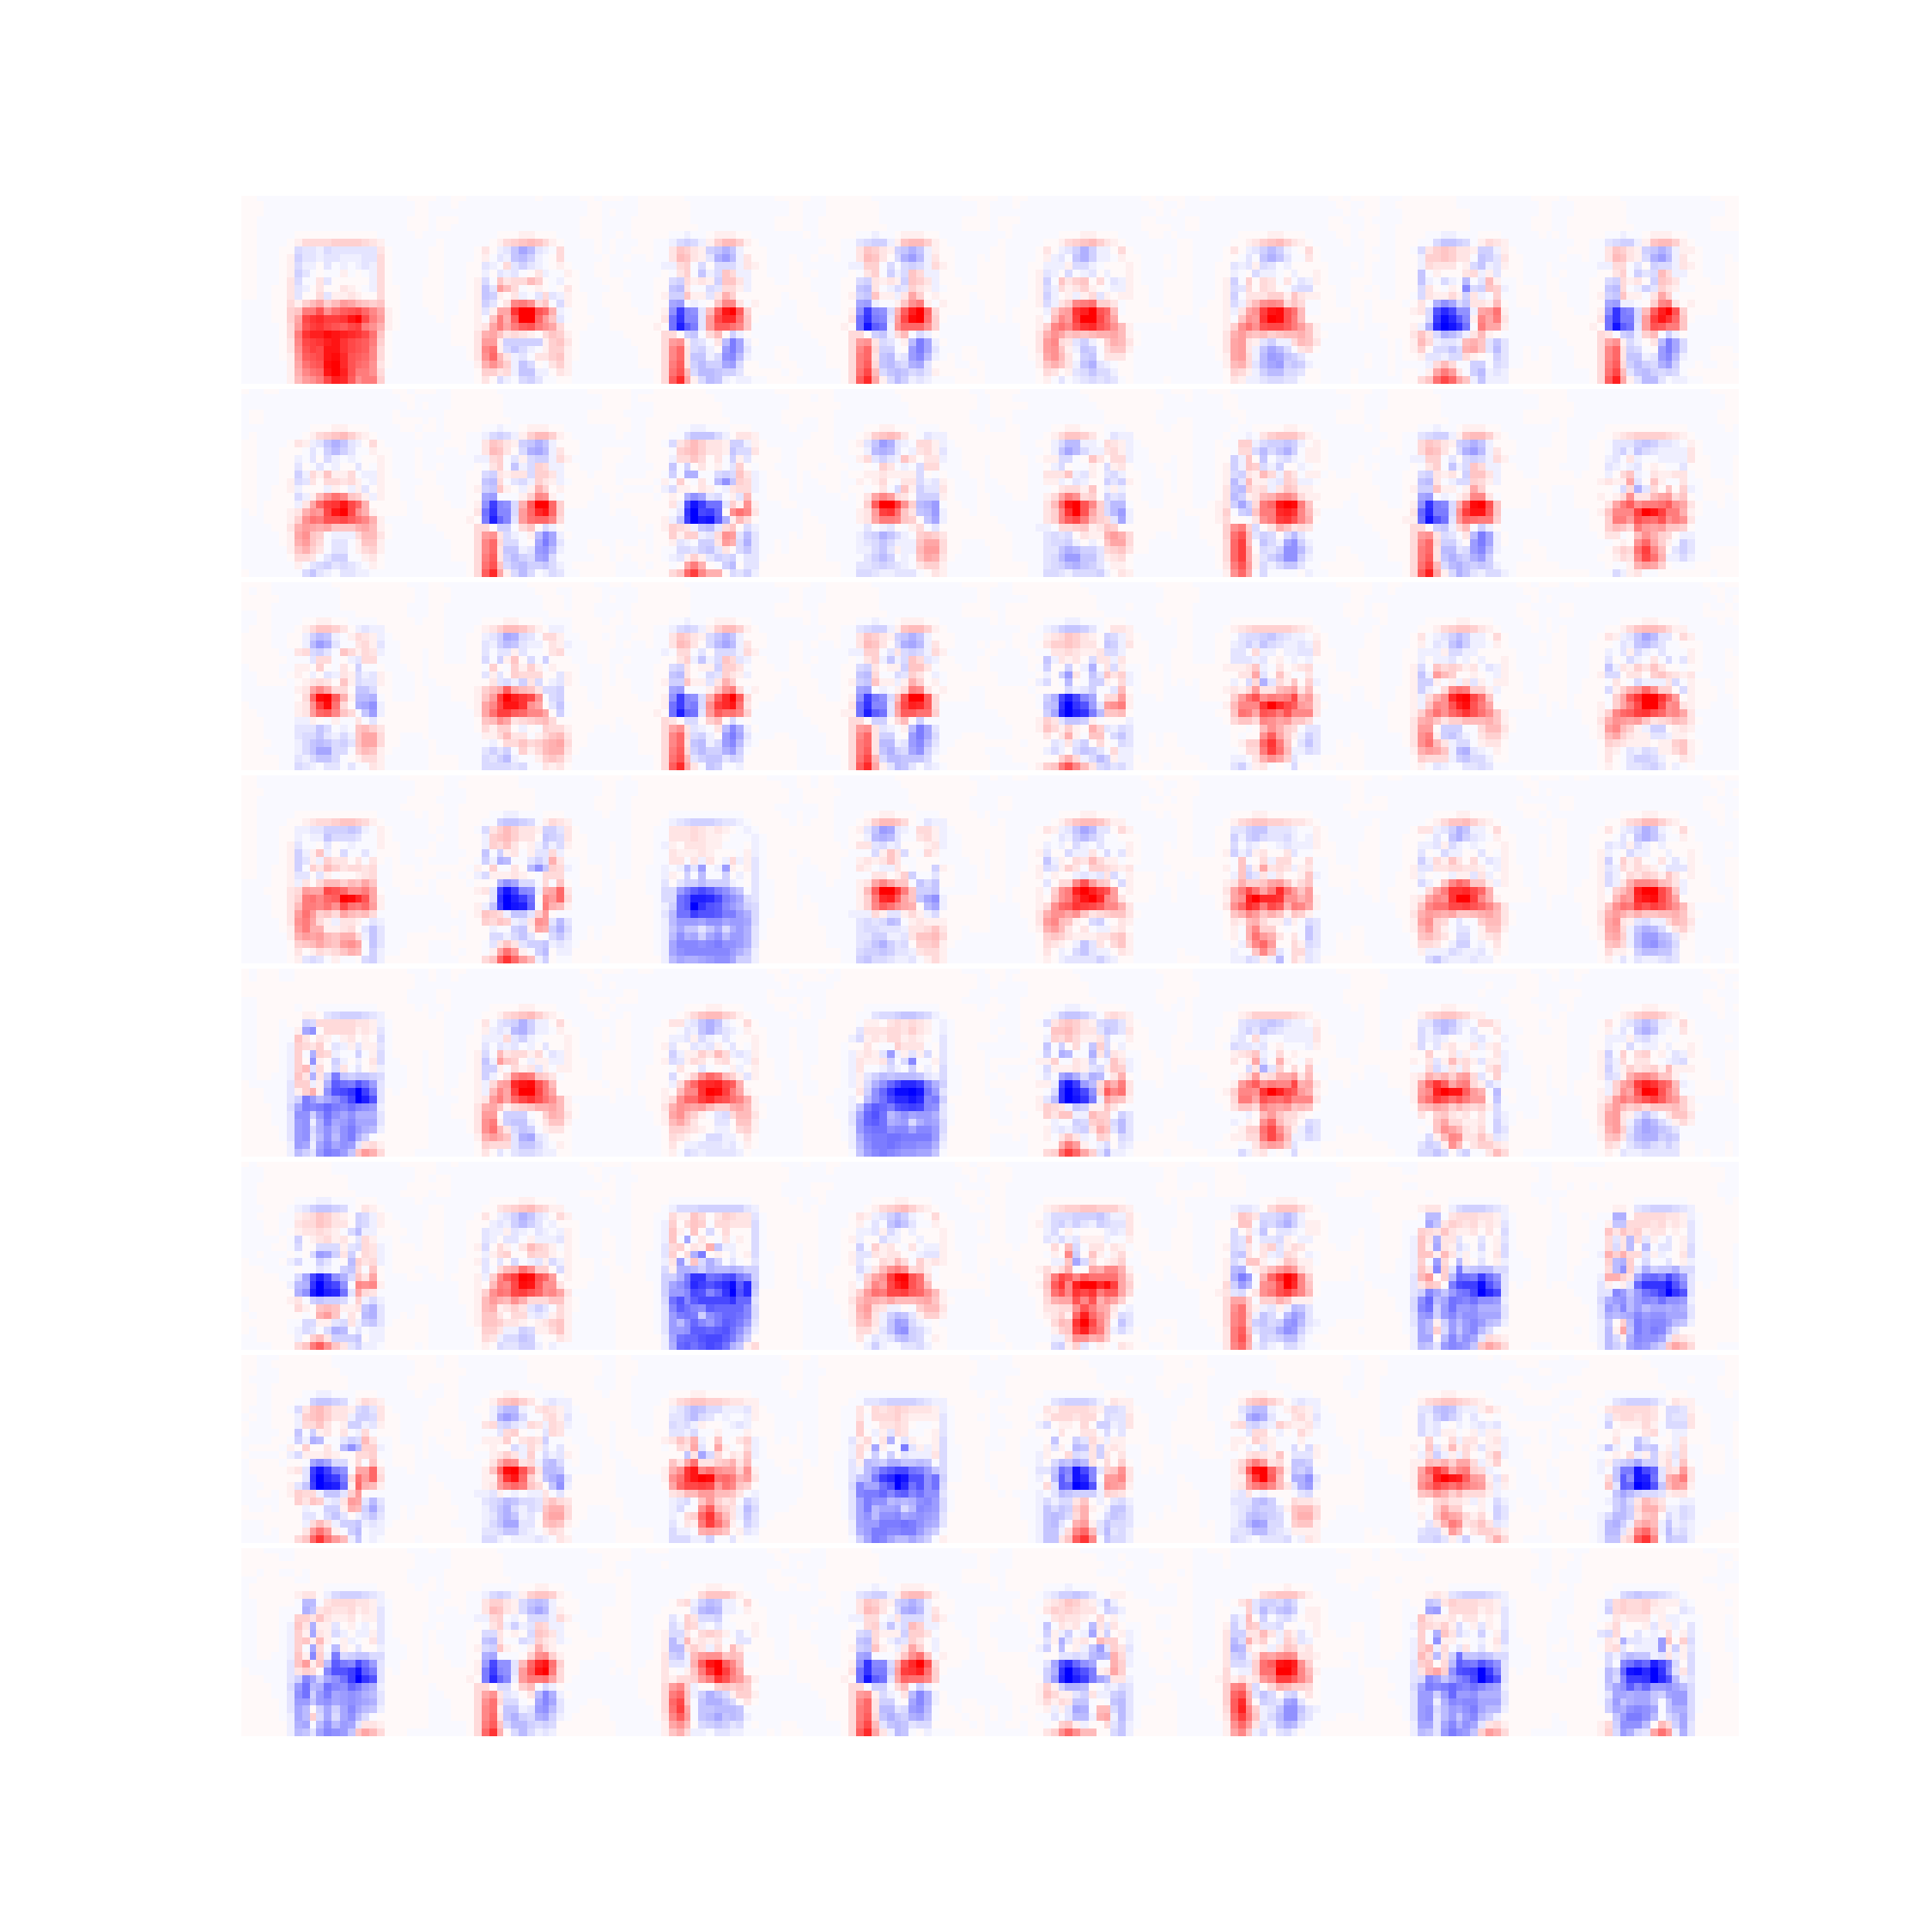
\includegraphics[width=0.95\textwidth]{figures/conv-diffs-ben-window.pdf}
  \caption{caption}
  \label{fig:convkernelsWindow}
\end{figure}
% subsubsection understanding_what_we_learn (end)

% subsection small_window_studies (end)





% section studies (end)


\section{Acknowledgements}

This work is supported by the US Department of Energy (DOE) Early Career Research Program and grant DE-AC02-76SF00515. BN is supported by the NSF Graduate Research Fellowship under Grant No. DGE-4747 and by the Stanford Graduate Fellowship.  SDSI?

% \nocite{*}



% \bibliography{myrefs}





\end{document}
